% !TEX root = ./informe.tex
\newpage
\section{Comparativas}
Nuestro análisis de las heurísticas se centra en evaluar dos aspectos de las mismas: el tiempo requerido para ejecutarse y la cantidad promedio de conflictos que aparecen en la solución.


Nuestros test se basan en grafos generados de distintas maneras:

Por un lado generamos grafos completamente al azar, de los cuales no se conoce a priori si son coloreables o no (determinar si un grafo genérico tiene coloreo requiere un tiempo no polinomial, lo cual resulta impracticable para grafos grandes). Estos test, además de ser útiles para medir el tiempo de ejecución, también permiten analizar los resultados de las heurísticas de búsqueda local, ya que permiten detectar conflictos reportados por el goloso, que luego fueron corregidos por las otras heurísticas.

Por otro lado, para otros tests, utilizaremos grafos bipartitos completos, de los cuales tenemos la certeza de que son coloreables (ya que esta demostrado que todo grafo bipartito es coloreable utilizando dos colores). Estos grafos bipartitos se construyeron de manera que dos colores específicos están presentes como alternativas en todos los nodos,  y adicionalmente se agregaron otros colores elegidos al azar para cada nodo. De esta forma, se esta asegurando que existe al menos una solución de coloreo válida para todos los grafos bipartitos generados. Este coloreo consistiría en seleccionar el primer color que los nodos tienen en común para uno de los subconjuntos de vértices del grafo bipartito, y el otro color para el otro subconjunto.

Pensamos que los grafos bipartitos generados para los tests, aunque son un caso particular, pueden resultar interesantes para el análisis de la cantidad de conflictos de las heurísticas. Son grafos de los cuales se tiene la certeza de que son coloreables, pero que igualmente pueden contener una cantidad elevada de nodos y aristas.

A continuación se exponen los gráficos generados a partir de los resultados de los experimentos que ideamos e implementamos con el fin de hacer un análisis empírico del costo temporal y la calidad de los resultados obtenidos a partir del algoritmo goloso (Ejercicio 3) y de la vecindad 1 del algoritmo de búsqueda local (Ejercicio 4).

Para ello, separamos este apartado en la observación de tres conjuntos de resultados:

\begin{itemize}
\item {Los obtenidos a partir de grafos completos}
\item {Los obtenidos a partir de grafos cíclicos}
\item {Los obtenidos a parir de grafos bipartitos completos}
\end{itemize}

Consideramos que hacerlo fue de especial relevancia, dado que al incrementar individualmente el valor de parámetros independientes es factible que se terminen realizando experimentos sobre grafos estructuralmente distintos, con poca o ninguna relación en cuanto a sus propiedades.\\
Los resultados se observan a continuación:\\


\subsection {Resultados obtenidos a partir de grafos cíclicos}

En las figuras \ref{TiempoGreedyCiclico} y \ref{TiempoLocalCiclico} se muestran los tiempos medidos para los distintos algoritmos en grafos cíclicos de distintos tamaños. \\
Observándolos en su conjunto, se puede apreciar que no sólo el algoritmo goloso se comporta de manera más uniforme en función de la entrada, si no que también se hace notorio que el mismo demanda un tiempo de cómputo mucho mayor en cada uno de los casos.\\

\begin{figure}[H]
    \centering
  	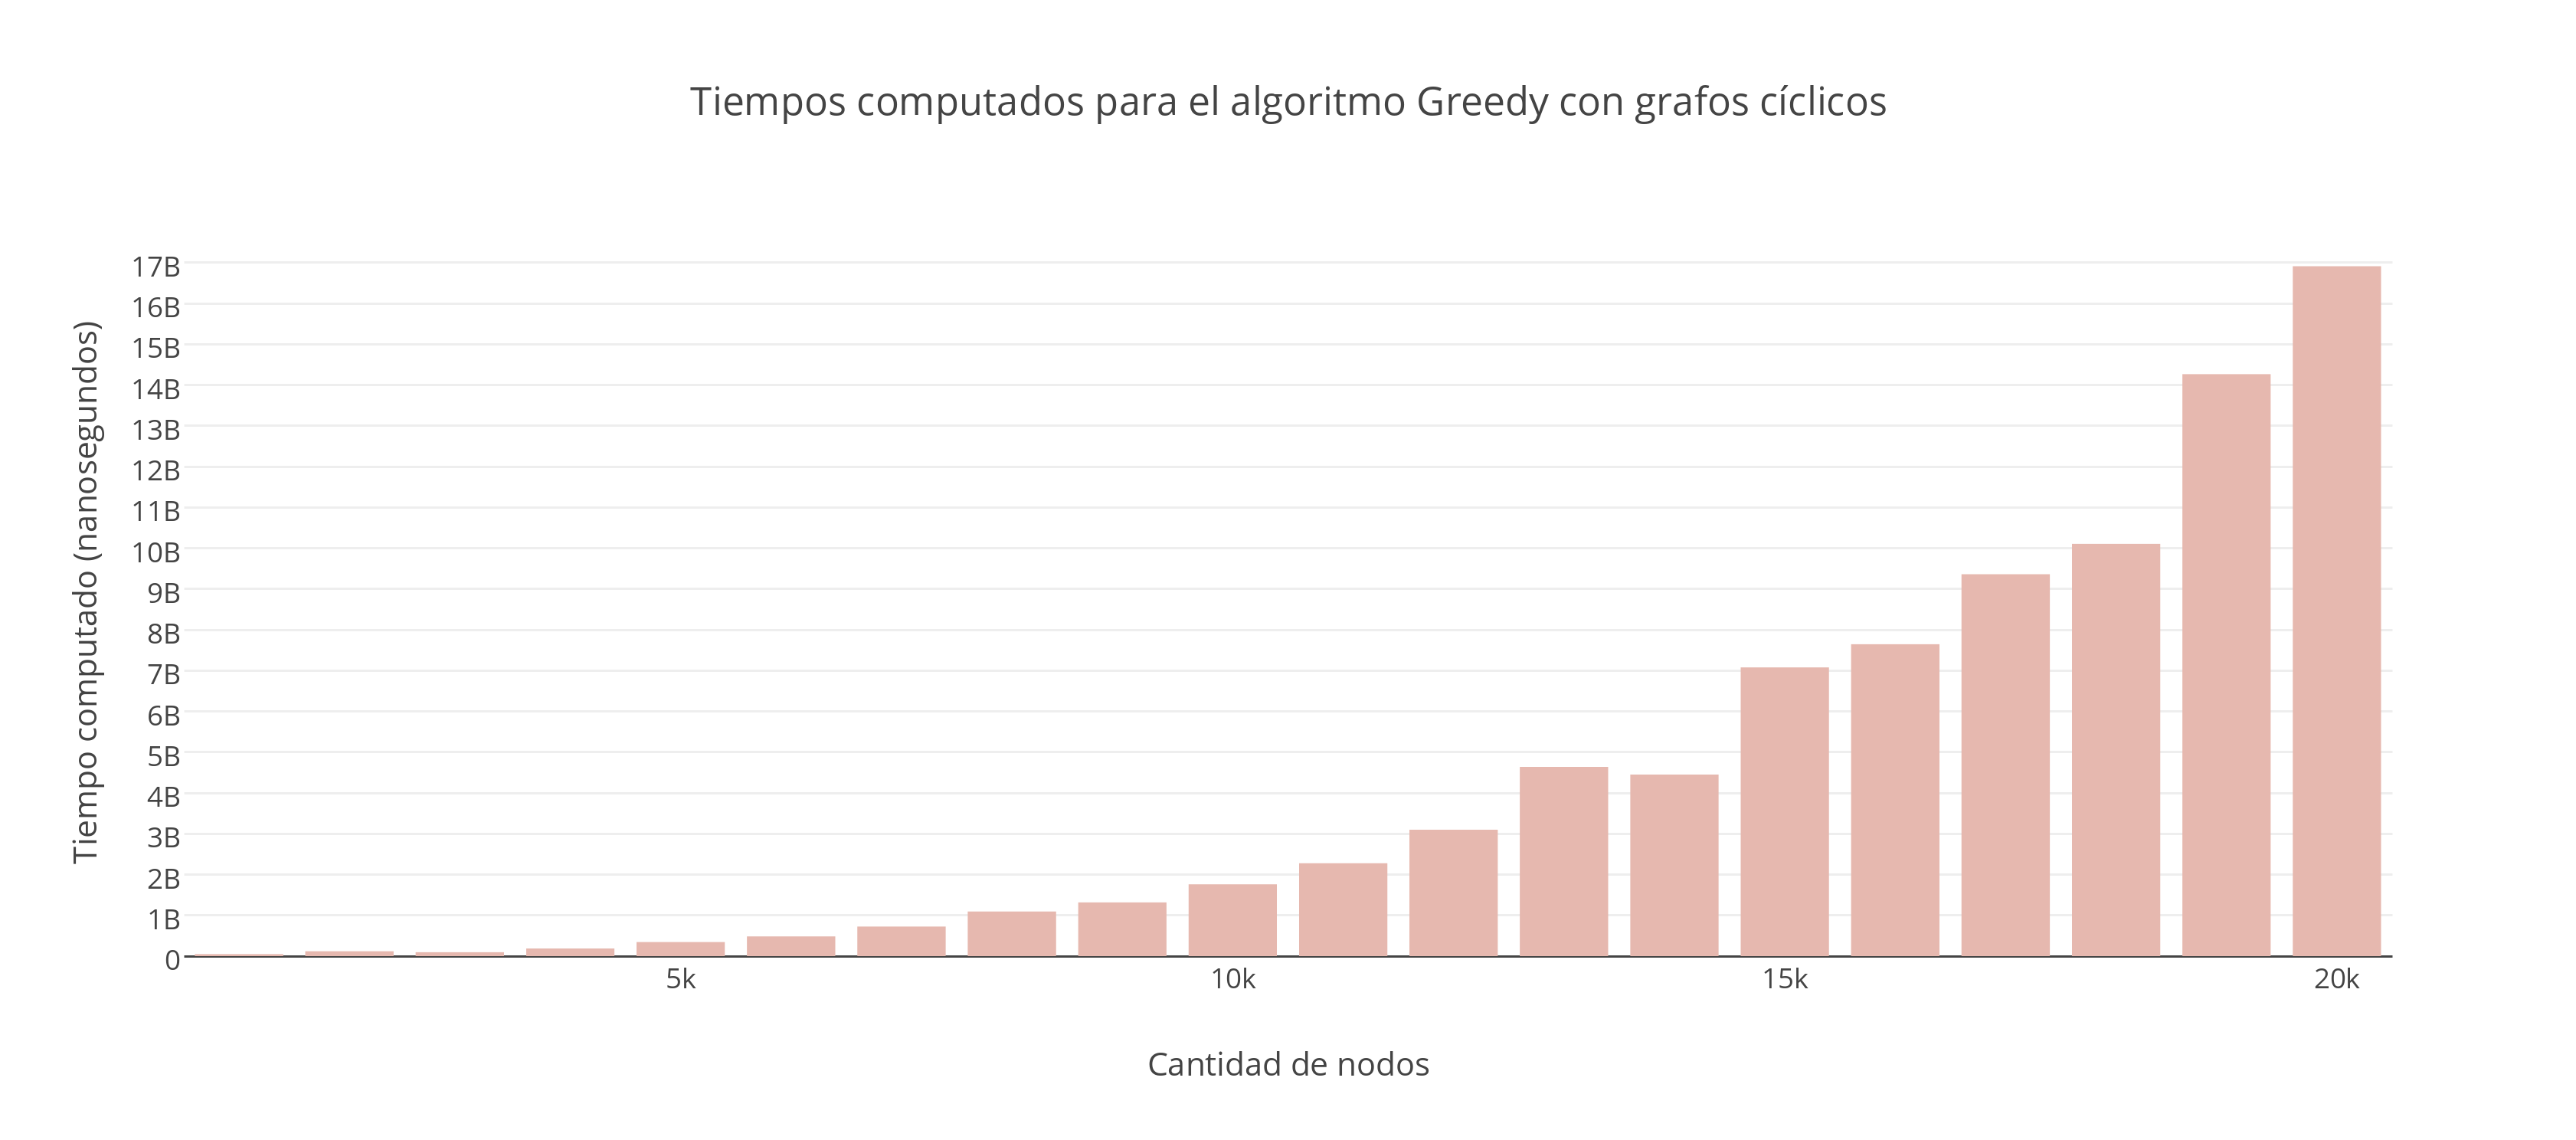
\includegraphics[width=18cm]{imagenes/Ej5/TiempoGreedyCiclico.png}
    \caption{}
 	  \label{TiempoGreedyCiclico}
  \end{figure}

 \begin{figure}[H]
    \centering
  	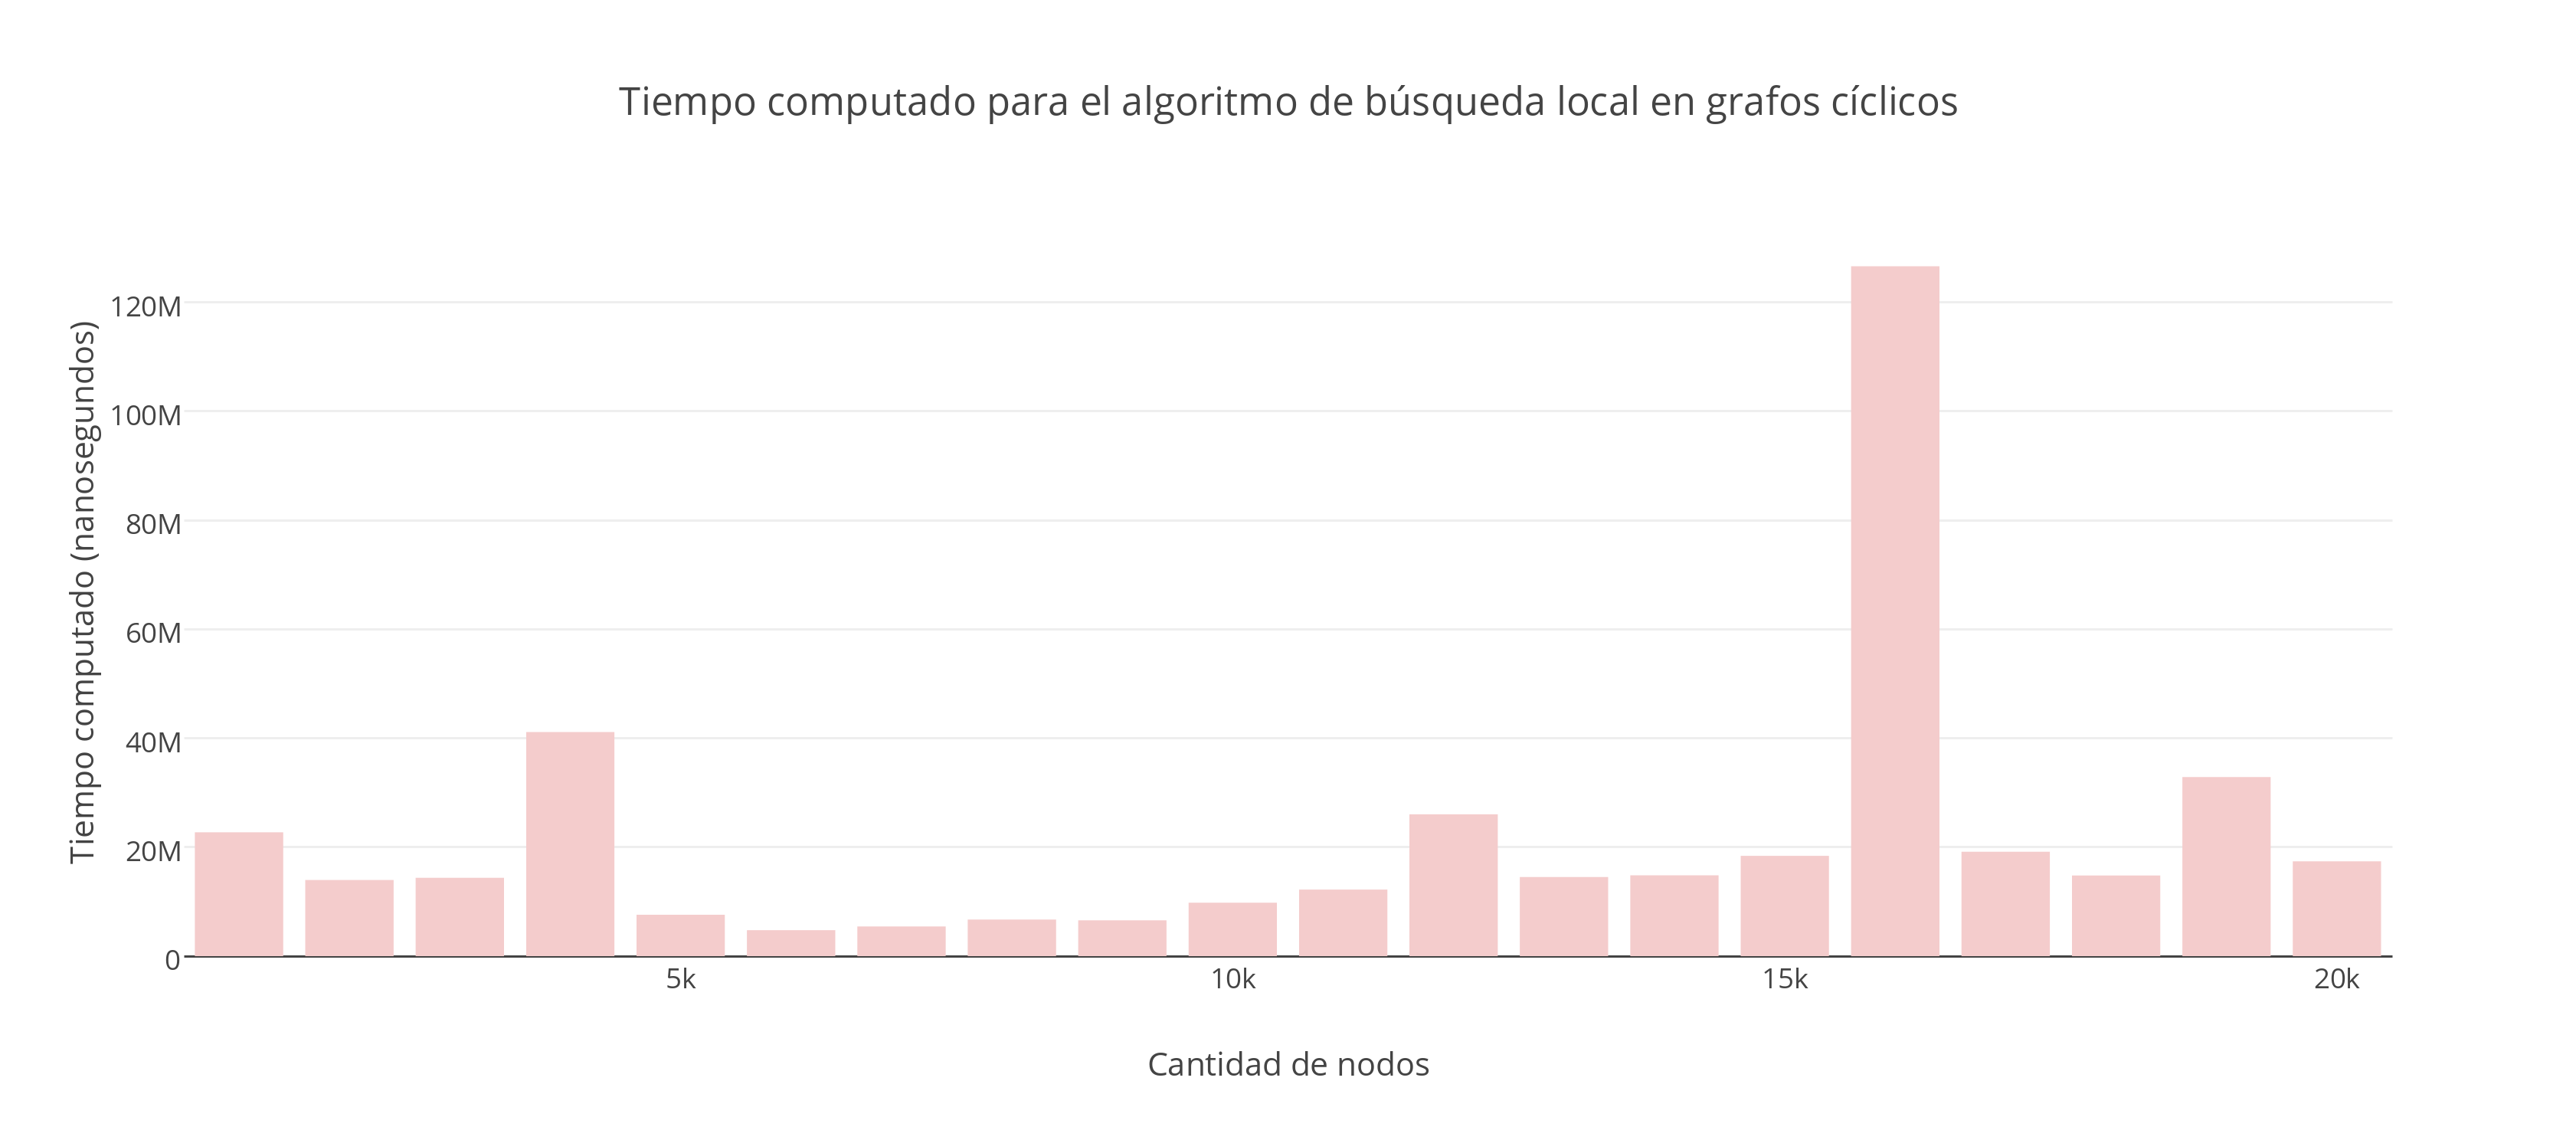
\includegraphics[width=18cm]{imagenes/Ej5/TiempoLocalCiclico.png}
    \caption{}
 	  \label{TiempoLocalCiclico}
  \end{figure}

Esto se manifiesta en la figura \ref{ComparacionTiemposCiclico}. Allí graficamos el porcentaje de tiempo ejecución de cada algoritmo para cada instancia en función del tiempo total de cómputo.\\
La comparativa se realizó de esta manera debido a que no son algoritmos que corran sobre instancias iguales: El algoritmo de búsqueda local busca mejorar un resultado ya obtenido por el algoritmo goloso y recibe nodos que se asumen bien coloreados de acuerdo a algún criterio prefijado.

 \begin{figure}[H]
    \centering
  	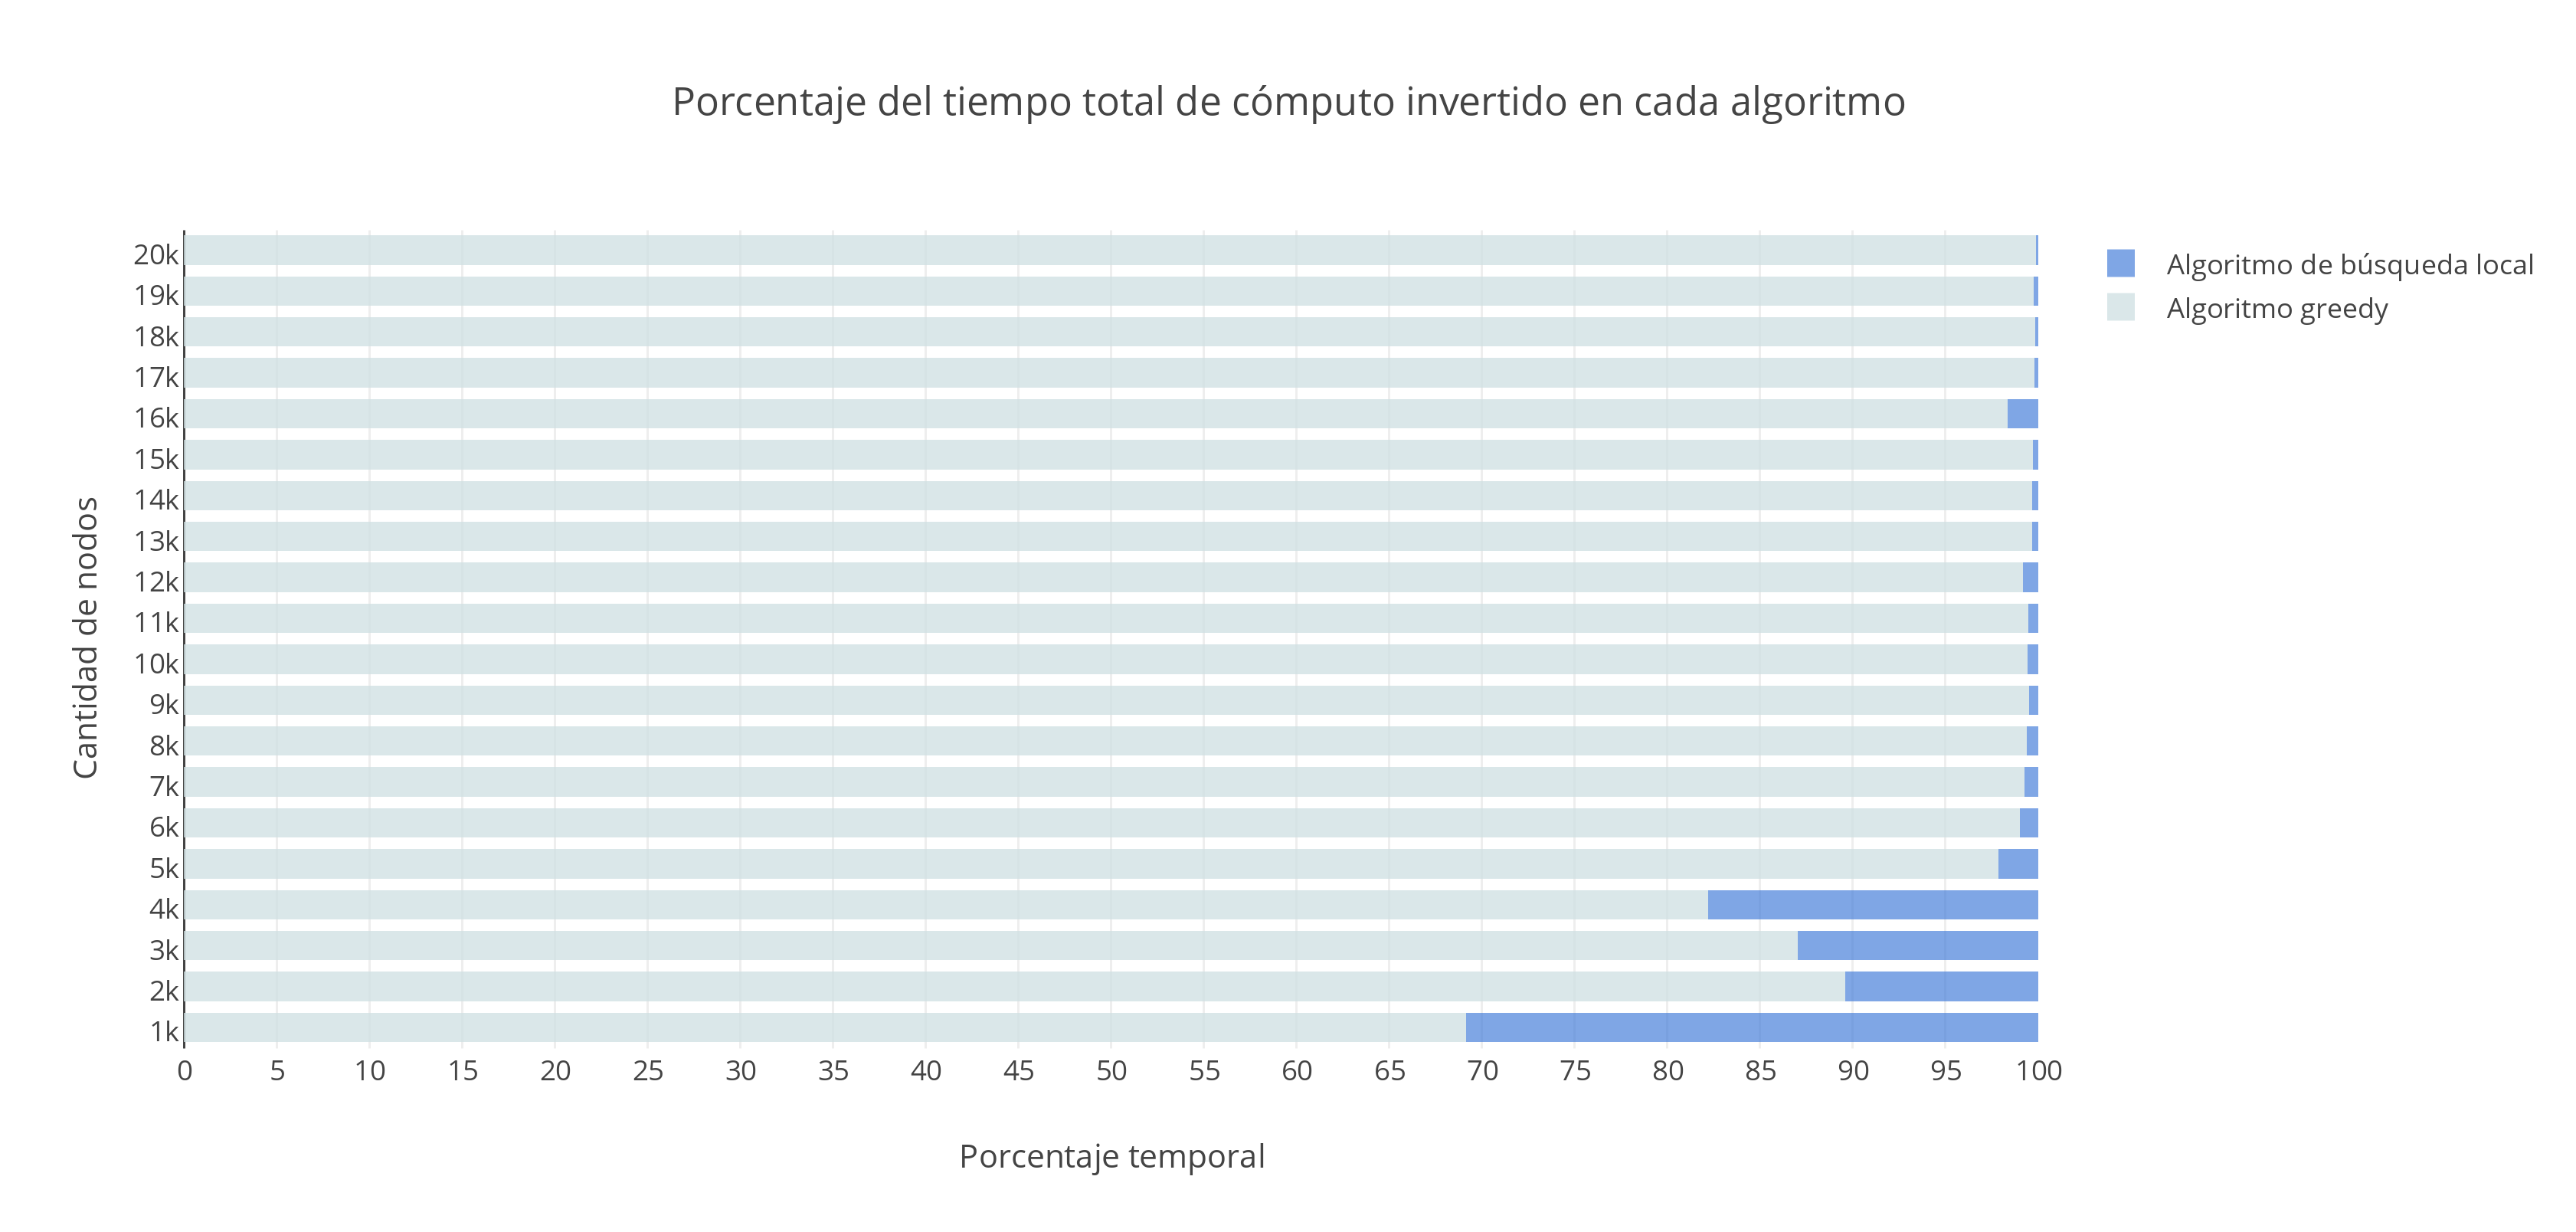
\includegraphics[width=18cm]{imagenes/Ej5/ComparacionTiemposCiclico.png}
    \caption{}
 	  \label{ComparacionTiemposCiclico}
  \end{figure}

Por último, el gráfico \ref{ComparacionConflictosCiclico} nos muestra que la cantidad de conflictos entre el output de los distintos algoritmos no varía notoriamente. Esto nos fuerza a concluir que en situaciones en las que se anticipa que el grafo pueda llegar a tener una estructura similar a uno cíclico y no sea estrictamente necesario conseguir un coloreo tan óptimo como sea posible, puede ser conveniente tomar los resultados arrojados por el primer algoritmo.

 \begin{figure}[H]
    \centering
  	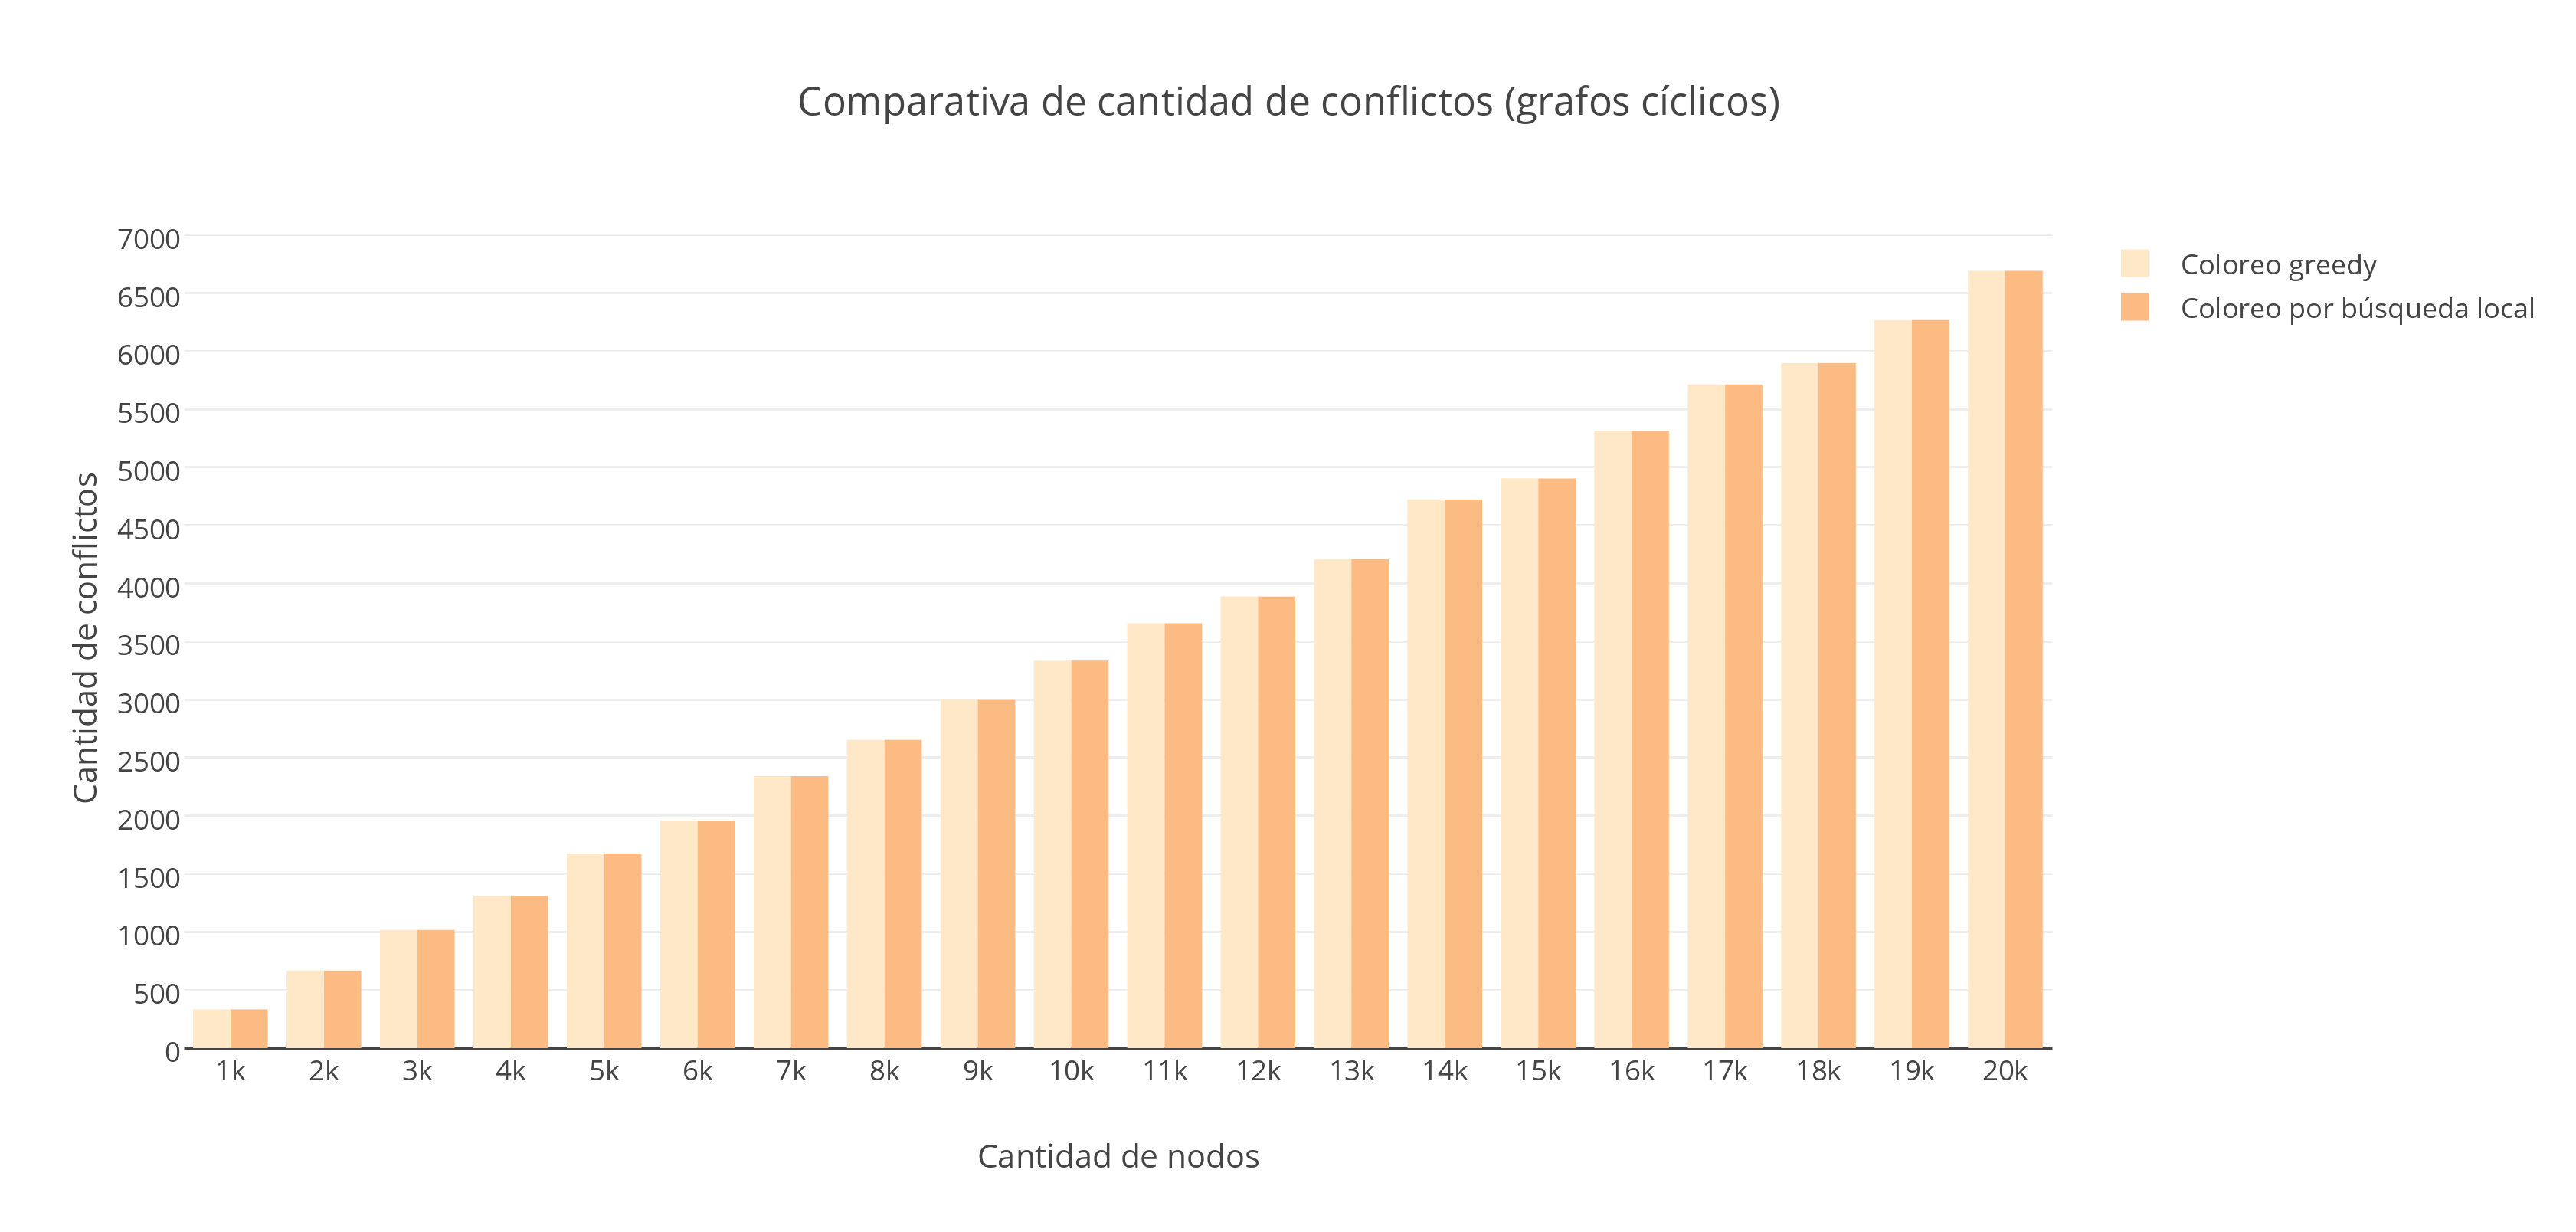
\includegraphics[width=18cm]{imagenes/Ej5/ComparacionConflictosCiclico.png}
    \caption{}
 	  \label{ComparacionConflictosCiclico}
  \end{figure}


\subsection {Resultados obtenidos a partir de grafos completos}

En las figuras \ref{TiempoGreedyCompleto} y \ref{TiemposLocalCompleto} muestran los tiempos (junto a sus cotas temporales) medidos observados para ambos algoritmos ejecutados sobre grafos completos de distintos tamaños.\\
Se hace realmente visible la diferencia en cuanto a costos temporales en la figura \ref{ComparacionTiemposCompleto}, en la cual se exhiben solapadas las barras que indican el tiempo de cómputo medido para cada algoritmo.

 \begin{figure}[H]
    \centering
  	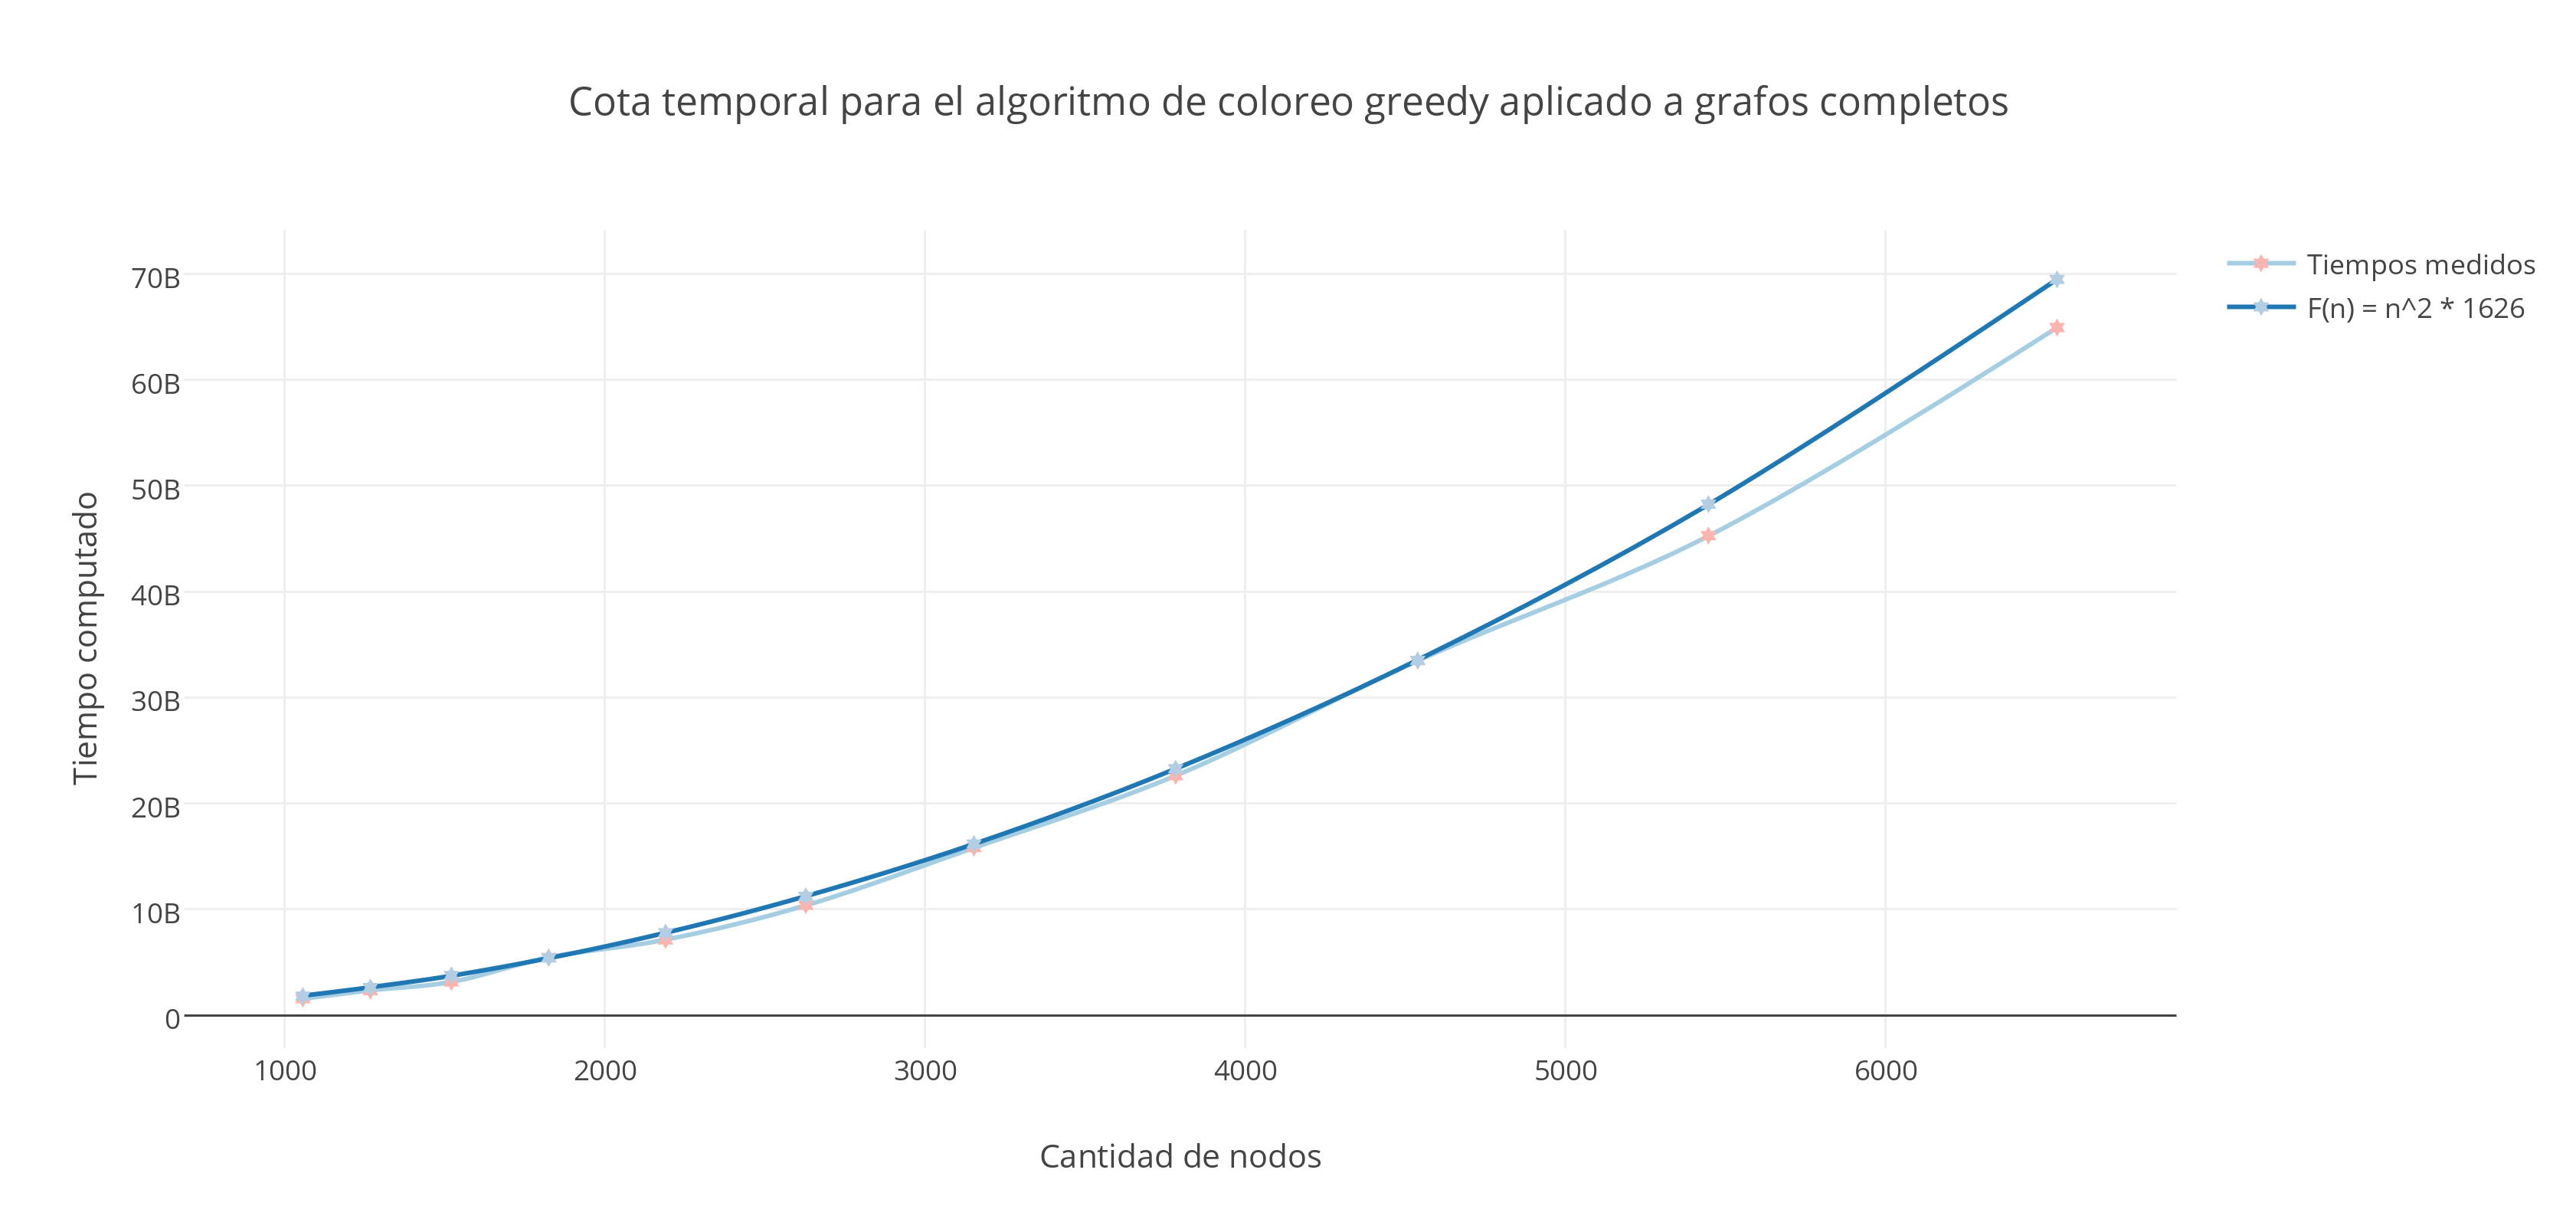
\includegraphics[width=18cm]{imagenes/Ej5/TiempoGreedyCompleto.png}
    \caption{}
 	  \label{TiempoGreedyCompleto}
  \end{figure}

 \begin{figure}[H]
    \centering
  	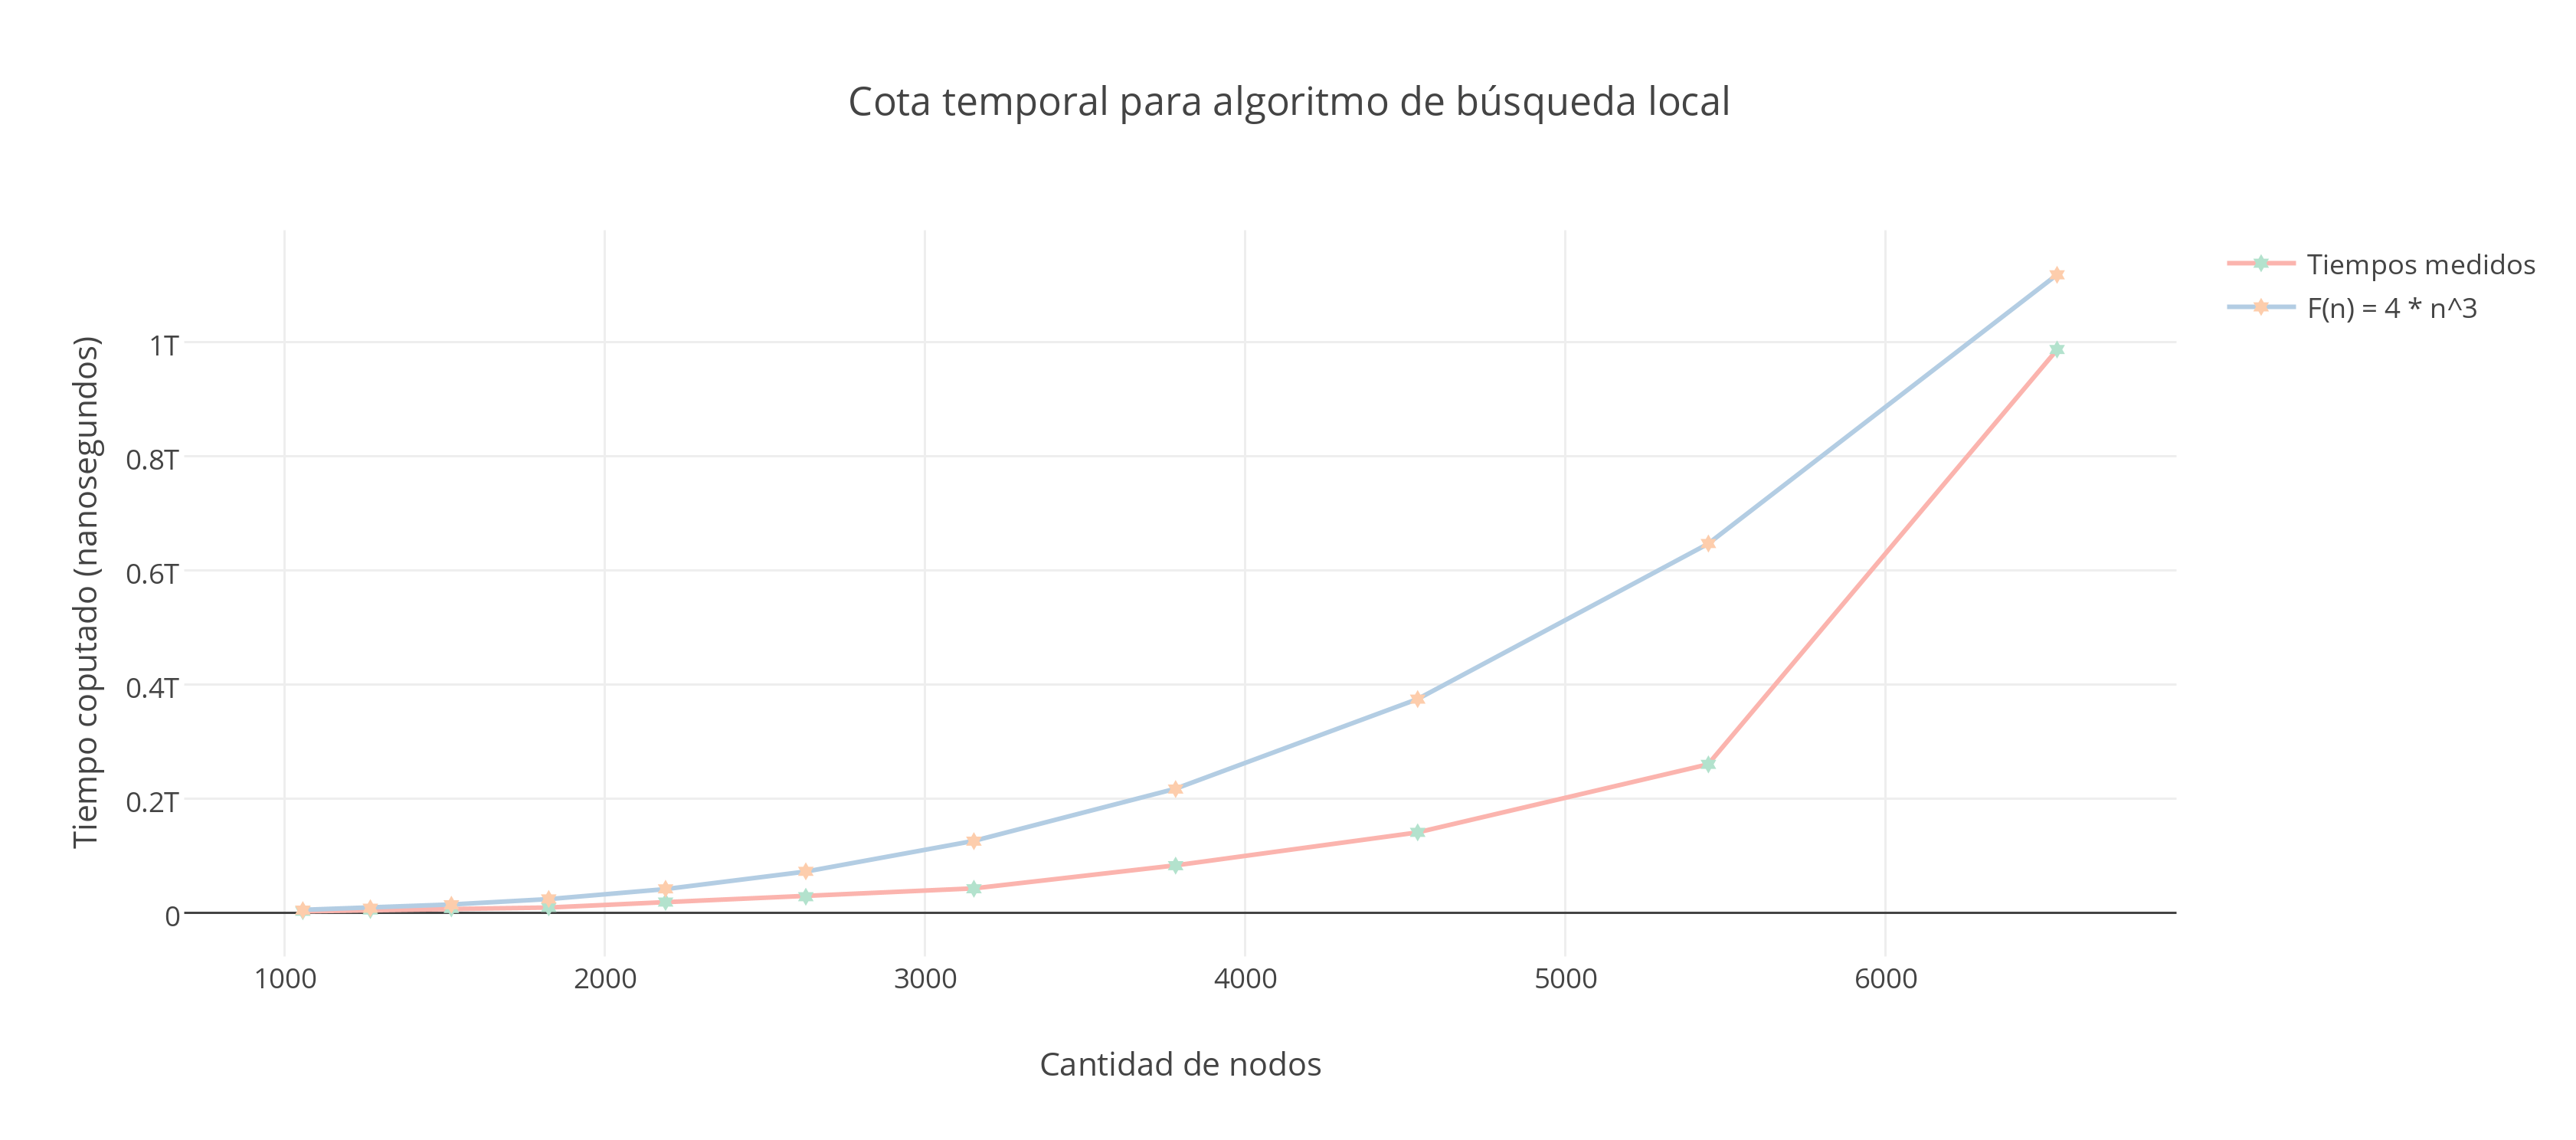
\includegraphics[width=18cm]{imagenes/Ej5/TiemposLocalCompleto.png}
    \caption{}
 	  \label{TiemposLocalCompleto}
  \end{figure}

 \begin{figure}[H]
    \centering
  	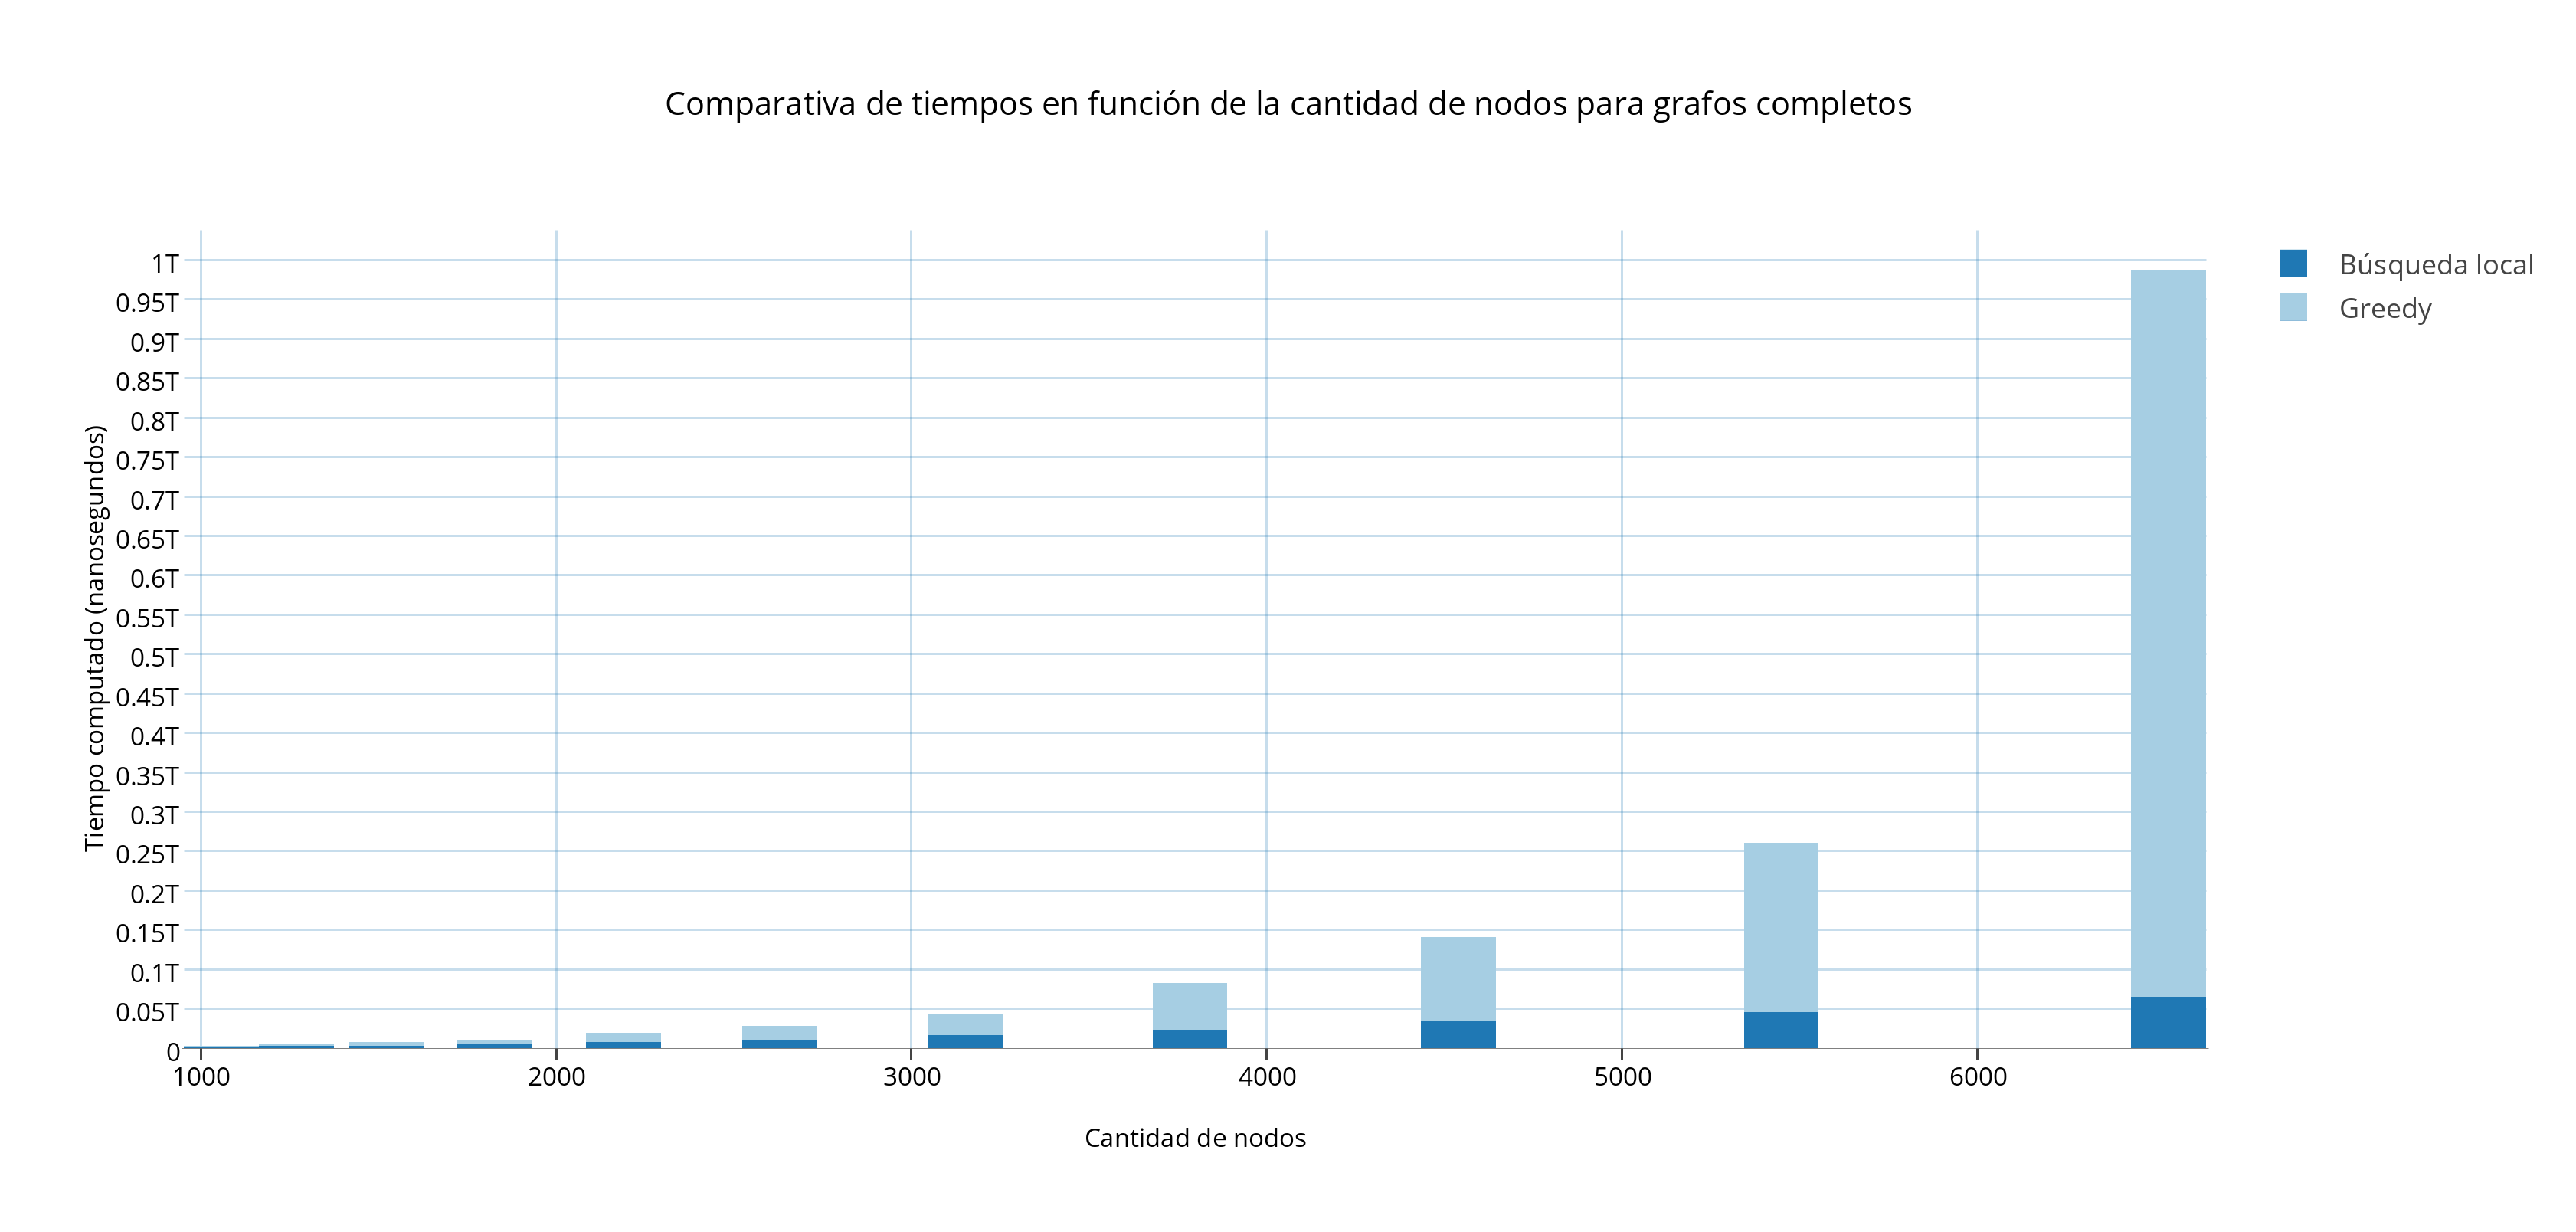
\includegraphics[width=18cm]{imagenes/Ej5/ComparacionTiemposCompleto.png}
    \caption{}
 	  \label{ComparacionTiemposCompleto}
  \end{figure}

Sin embargo, a diferencia de lo observado en la figura \ref{ComparacionConflictosCiclico}, en la ilustración \ref{ComparacionConflictosCompleto} puede apreciarse la disminución en la cantidad de conflictos resultante del posprocesamiento del grafo obtenido luego de la ejecución del algoritmo goloso.\\
Dicho esto, pareciera ser que en los casos en que el grafo no es esparzo, el algoritmo de búsqueda local si es una buena opción en términos del costo temporal y el beneficio cualitativo del resultado.

 \begin{figure}[H]
    \centering
  	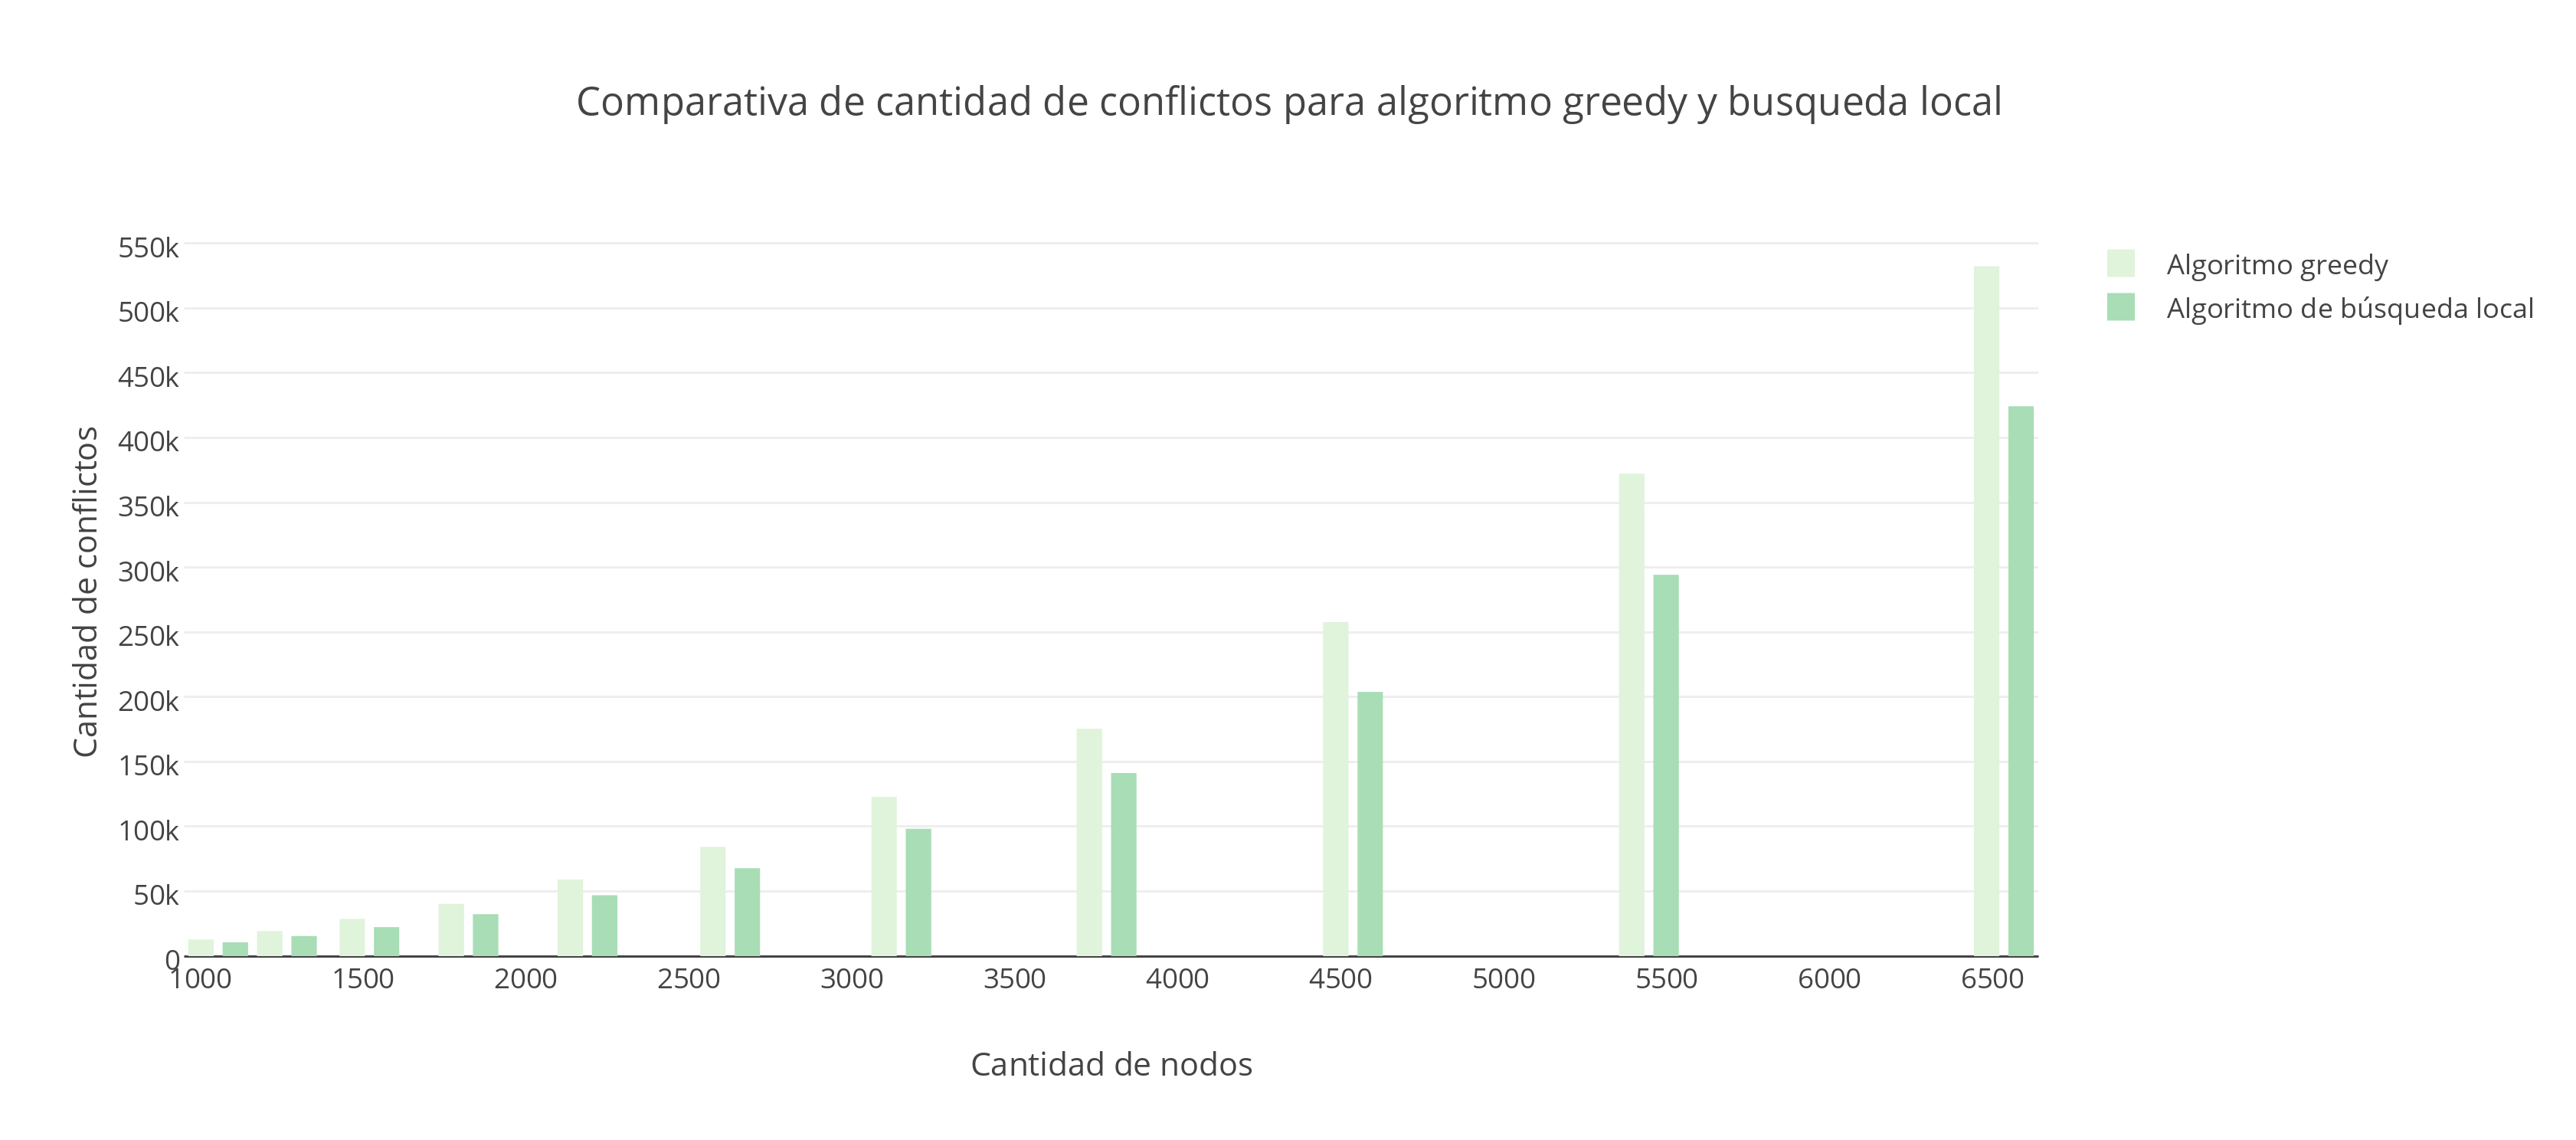
\includegraphics[width=18cm]{imagenes/Ej5/ComparacionConflictosCompleto.png}
    \caption{}
 	  \label{ComparacionConflictosCompleto}
  \end{figure}

\subsection {Resultados obtenidos a parir de grafos bipartitos completos}

Como se mencionó antes, la particularidad de esta familia de grafos es que se pueden colorear con dos colores si nos aseguramos de que cada nodo tenga al menos dos colores específicos. Por lo tanto analizaremos de que manera aprovechan estas propiedades las dos heurísticas.\\

Observando la figura \ref{TiemposGreedyBL} notamos que a diferencia con las otras familias de grafos analizadas, los tiempos de ejecución de \emph{Búsqueda Local} son considerablemente mayores a los del \emph{Goloso}.

\begin{figure}[H]
  \centering
  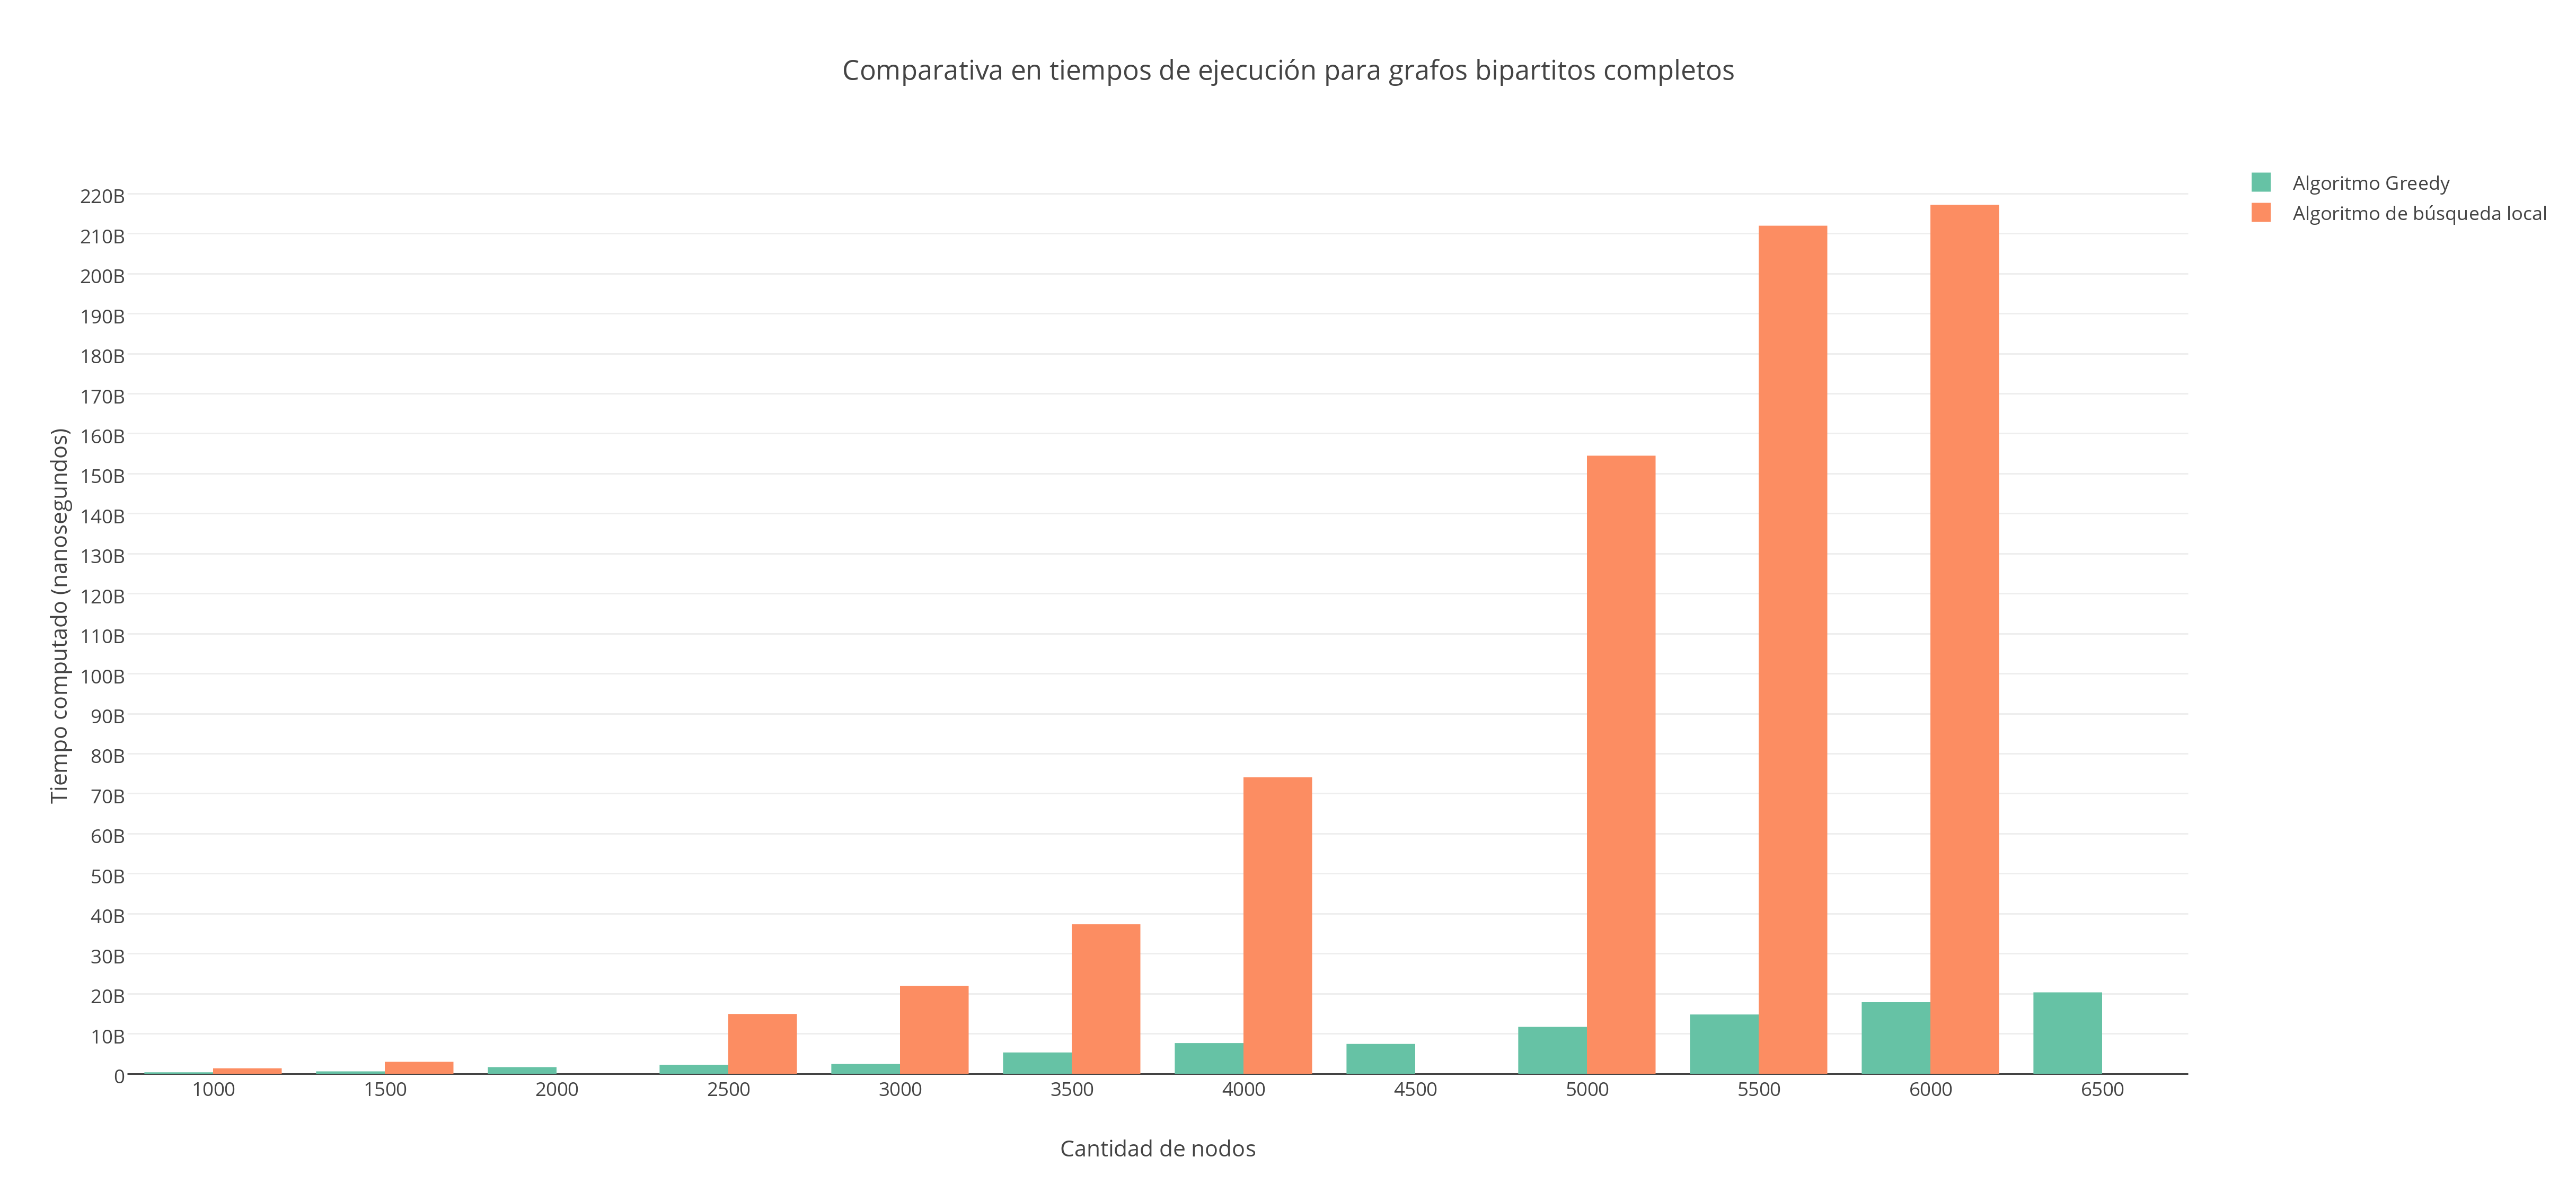
\includegraphics[width=18cm]{imagenes/Ej5/bipartitosCompletos/TiemposGreedyBL.png}
  \caption{}
    \label{TiemposGreedyBL}
\end{figure}

\begin{figure}[H]
  \centering
  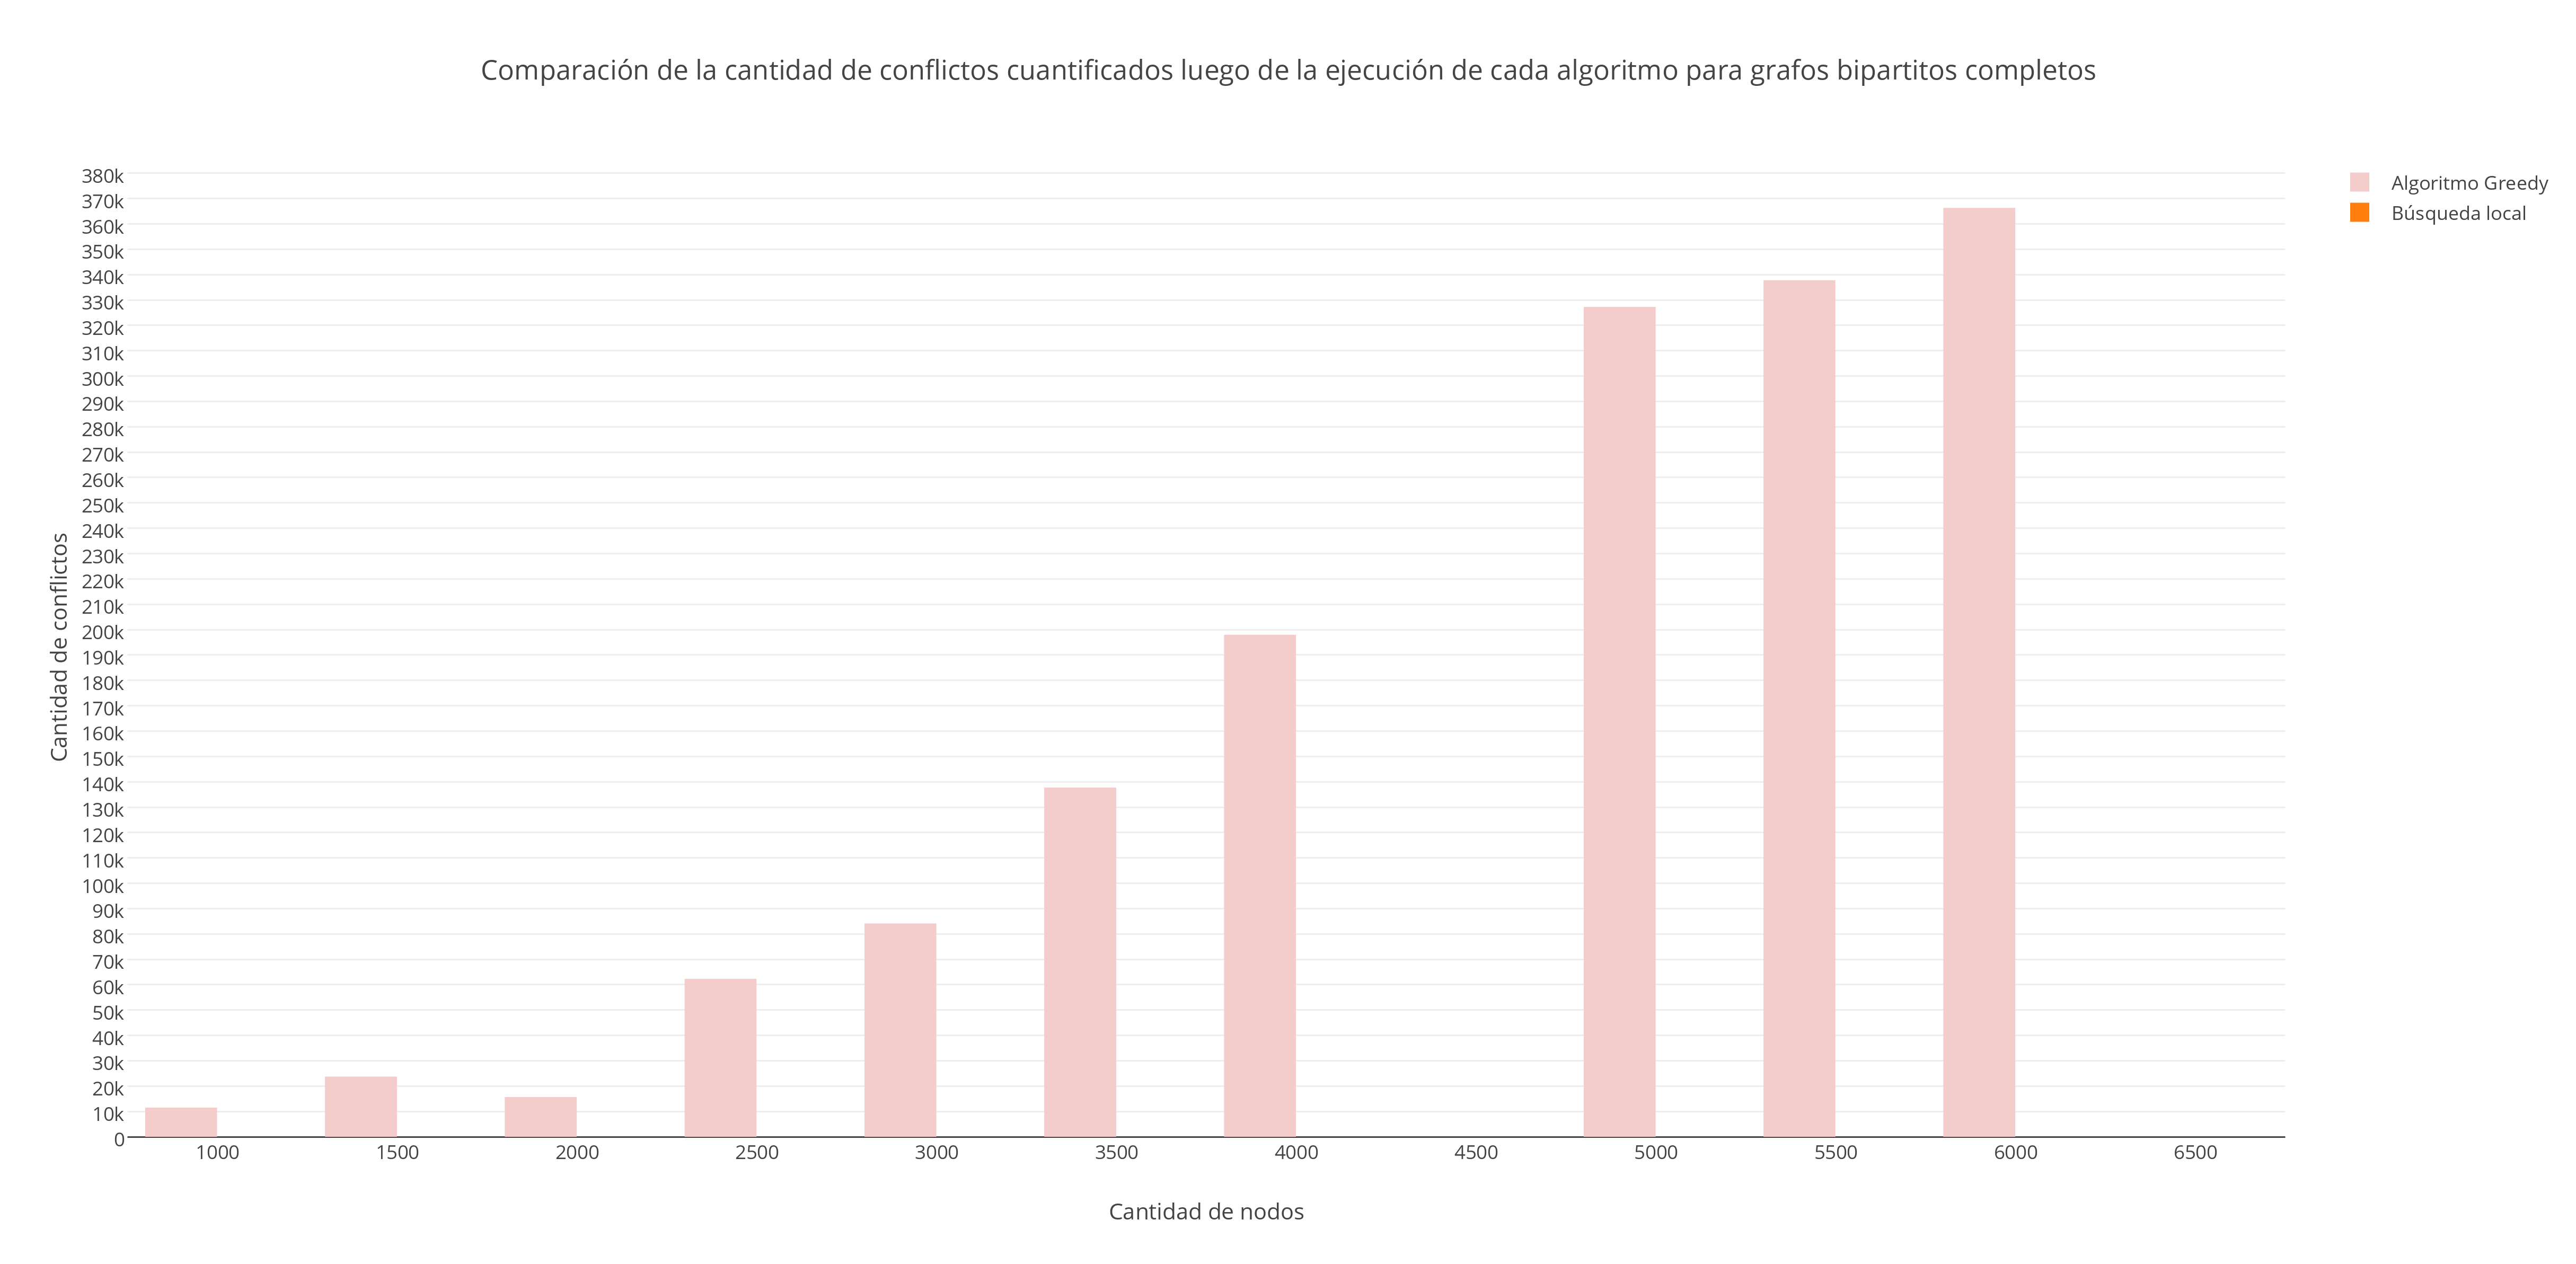
\includegraphics[width=18cm]{imagenes/Ej5/bipartitosCompletos/ConflictosGreedyBL.png}
  \caption{}
    \label{ConflictosGreedyBL}
\end{figure}

Por otra parte en la figura \ref{ConflictosGreedyBL} se puede ver que al comparar la cantidad final de conflictos, el greedy deja muchos sin resolver ya que por como se seleccionan los colores para cada nodo no puede darse cuenta de que es un grafo bipartito y no puede hacer uso de las propiedades del mismo para encontrar un coloreo. En contrapartida tenemos la búsqueda local, que al utilizar como entrada el grafo coloreado por el goloso, logra resolver todos los conflictos. Lo cual está directamente relacionado con que el tiempo de ejecución sea tanto mas grande porque si recordamos la complejidad de la vecindad 1 que era $\mathcal{O}(n + c)$ con $n$ nodos y $c$ conflictos, se deduce que a mayor cantidad de conflictos que deja el goloso sin resolver, mayor va a ser el tiempo que le tome resolverlos a la búsqueda local. Si miramos los gráficos \ref{TiemposGreedyBL} y \ref{ConflictosGreedyBL} se puede decir que, a misma cantidad de nodos, son comparables los tiempos de ejecución de la búsqueda local con la cantidad de conflictos sin resolver del goloso ya que se elevan casi en igual medida.\\

Por último, en la figura \ref{ConfTiempoBL} graficamos la cantidad de conflictos resueltos por el algoritmo de búsqueda local en función del tiempo. Al igual que antes se puede ver que a mayor cantidad de conflictos, mayor tiempo de cómputo. Por lo cual para esta familia de grafos específicamente si se busca obtener una solución exacta, se podría utilizar el algoritmo de búsqueda local como alternativa al backtracking, pero si lo que se busca es una aproximación en poco tiempo, se debería usar el goloso.

\begin{figure}[H]
  \centering
  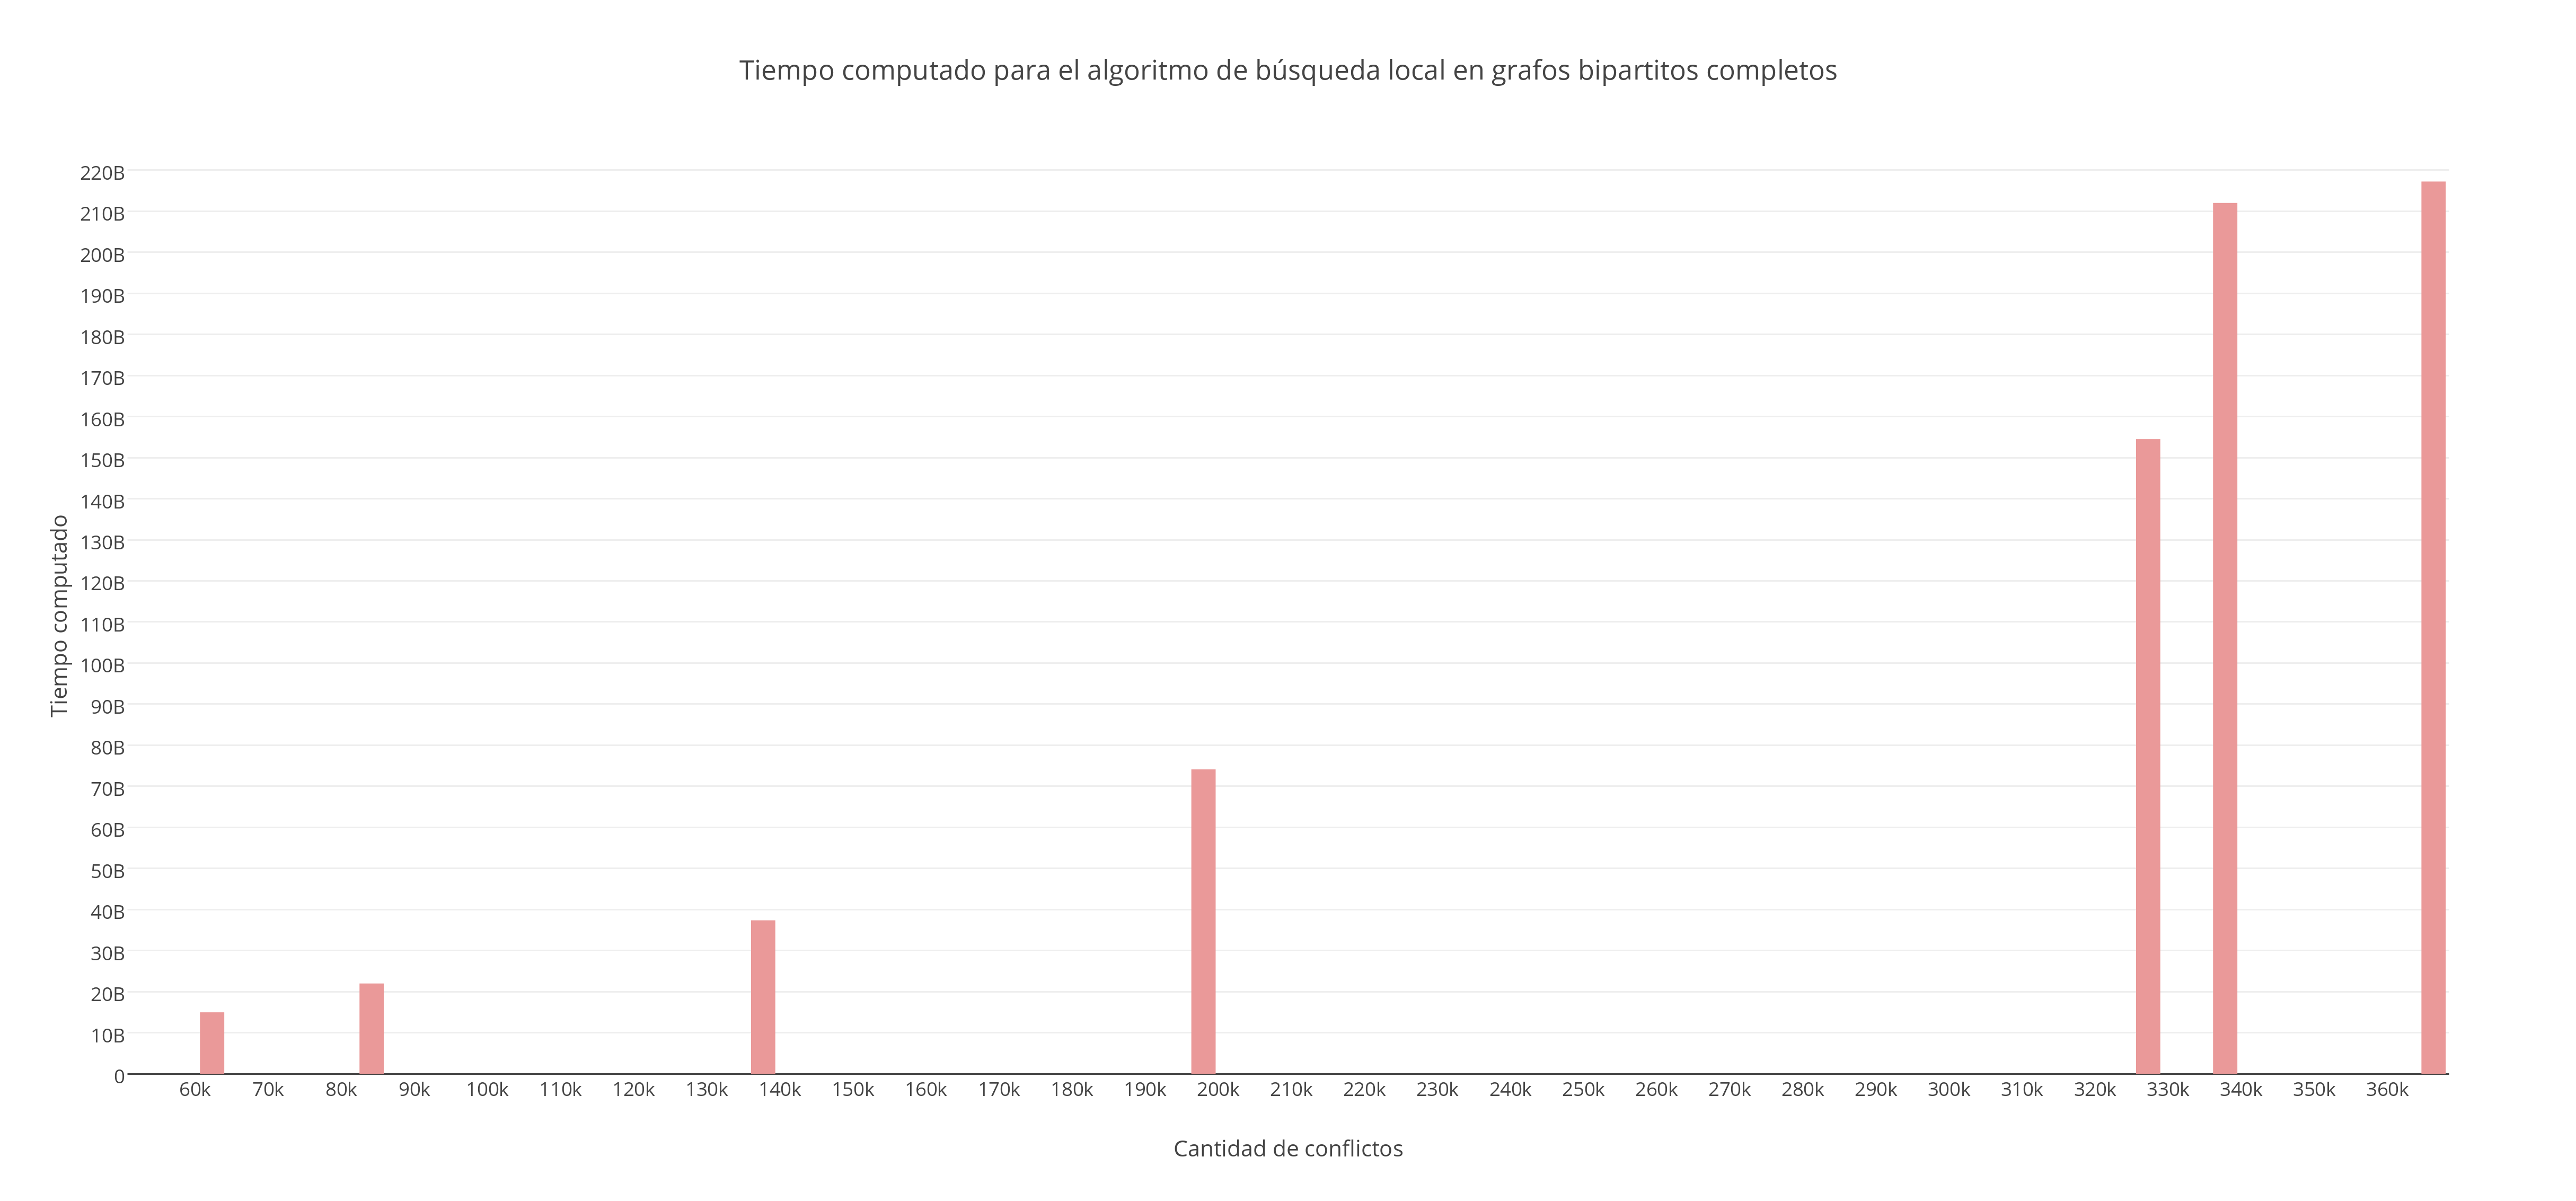
\includegraphics[width=18cm]{imagenes/Ej5/bipartitosCompletos/ConfTiempoBL.png}
  \caption{}
    \label{ConfTiempoBL}
\end{figure}

En conclusión, luego de examinar estos tres aspectos, creemos que a la hora de elegir utilizar una heurística, es conveniente analizar los resultados de las distintas opciones para determinar cual se adapta mejor a los resultados que estamos buscando. Ya que si bien la búsqueda local en general obtuvo mejoras en menos tiempo que el goloso, no hay que olvidarse que para obtener esas mejoras se corrió el goloso antes. Por lo tanto es bueno saber estos resultados a la hora de elegir, para poder priorizar las características que mas nos importa reforzar, ya se que de un coloreo rápido, que minimice los conflictos, que se aproxime mas a un resultado exacto, etc.
